\documentclass[11pt,a4paper]{article}
\usepackage[a4paper,margin=2.2cm]{geometry}
\usepackage{fontspec}
\setmainfont{Noto Serif CJK TC}[BoldFont={Noto Serif CJK TC Bold}]
\setsansfont{Noto Sans CJK TC}[BoldFont={Noto Sans CJK TC Bold}]
\XeTeXlinebreaklocale "zh"
\XeTeXlinebreakskip = 0pt plus 1pt
\usepackage{amsmath,amssymb,bm}
\usepackage{tabularx,booktabs,array}
\usepackage{enumitem}
\usepackage[most]{tcolorbox}
\usepackage{xcolor}
\usepackage{graphicx}
\usepackage{hyperref}
\hypersetup{colorlinks=true,linkcolor=blue!50!black}
\setlength{\parindent}{0pt}
\setlength{\parskip}{0.5em}
\renewcommand{\arraystretch}{1.35}
\emergencystretch=3em
\binoppenalty=200\relpenalty=100

\definecolor{bluebg}{HTML}{F5F8FB}  \definecolor{blueframe}{HTML}{AFC0D2}  \definecolor{bluetitle}{HTML}{1F3864}
\definecolor{greenbg}{HTML}{F3F9F4} \definecolor{greenframe}{HTML}{A8CDB1} \definecolor{greentitle}{HTML}{1E5631}
\definecolor{redbg}{HTML}{FCF4F4}   \definecolor{redframe}{HTML}{DDB1B1}   \definecolor{redtitle}{HTML}{8B1E1E}
\definecolor{amberbg}{HTML}{FCF8EE} \definecolor{amberframe}{HTML}{DCC896} \definecolor{ambertitle}{HTML}{7A5200}
\definecolor{graybg}{HTML}{F6F6F6}  \definecolor{grayframe}{HTML}{C4C4C4}  \definecolor{graytitle}{HTML}{333333}
\newcommand{\boxmark}{\rule[0.02em]{0.62em}{0.62em}}
\tcbset{
  boxblue/.style ={colback=bluebg, colbacktitle=bluebg, colframe=blueframe, coltitle=bluetitle},
  boxgreen/.style={colback=greenbg,colbacktitle=greenbg,colframe=greenframe,coltitle=greentitle},
  boxred/.style  ={colback=redbg,  colbacktitle=redbg,  colframe=redframe,  coltitle=redtitle},
  boxamber/.style={colback=amberbg,colbacktitle=amberbg,colframe=amberframe,coltitle=ambertitle},
  boxgray/.style ={colback=graybg, colbacktitle=graybg, colframe=grayframe, coltitle=graytitle},
  notebox/.style={enhanced,breakable,sharp corners,boxrule=0.6pt,titlerule=0pt,
    fonttitle=\bfseries\large,toptitle=6pt,bottomtitle=2pt,
    left=10pt,right=10pt,top=4pt,bottom=8pt,before skip=10pt,after skip=12pt,
    boxblue}}
\newtcolorbox{cbox}[2][boxblue]{notebox,#1,title={\boxmark\enspace #2}}
\newtcolorbox{takeaway}[1][重點提示]{notebox,boxamber,title={\boxmark\enspace #1}}
\newtcolorbox{derivationbox}[1][完整推導]{notebox,boxblue,title={\boxmark\enspace #1}}
\newtcolorbox{trapbox}[1][常見陷阱]{notebox,boxred,title={\boxmark\enspace #1}}
\newtcolorbox{recipebox}[1][解題流程]{notebox,boxgreen,title={\boxmark\enspace #1}}

% ===== 記號 =====
\newcommand{\pl}{\mathbin{\|}}
\newcommand{\OD}[1]{V_{\text{OD}#1}}
\newcommand{\Vsq}[1]{\overline{V^2_{n,\text{#1}}}}
% ===== 例題標示 =====
\definecolor{extag}{HTML}{3A3A3A}
\definecolor{extagbg}{HTML}{E4E4E4}
\newcommand{\extag}[1]{\colorbox{extagbg}{\textcolor{extag}{\sffamily\bfseries\,例 #1\,}}}
\newcommand{\exhead}[3]{\par\medskip\noindent\extag{#1}\enspace{\bfseries #3}\enspace{\small\color{black!55}(p.#2)}\par\nopagebreak\smallskip}
\newcommand{\exref}[1]{\textcolor{extag}{\textbf{\sffamily 例 #1}}}
\newcommand{\rfig}[3]{\begin{center}\begin{minipage}{\linewidth}\centering\includegraphics[width=#2\linewidth]{../fig/ch9/fig9_#1.png}\\[0.1em]{\small\sffamily 圖 9.#1\quad #3}\end{minipage}\end{center}}

\begin{document}
\begin{center}{\LARGE\bfseries\sffamily ECD 單元複習講義：Operational Amplifiers（運算放大器）}\\[0.3em]{\large Razavi, \emph{Design of Analog CMOS Integrated Circuits}, 2nd ed., Ch.~9（pp.~344--409）}\end{center}

\textbf{記號約定}：$\OD{j}=V_{GS,j}-V_{TH,j}$ 表示 $M_j$ 的 overdrive（PMOS 取絕對值）；$V_{I_{SS}}$ 是尾電流源所需的最小跨壓（通常就是一個 overdrive）；$a\pl b$ 表示並聯。單級放大器的低頻增益一律寫成 $|A_v|=G_mR_{out}$（$G_m$ 為輸出短路時的轉導，$R_{out}$ 為輸出阻抗）。$\gamma$ 在本章有兩種意思：電路題中「$\gamma=0$」通常是 \textbf{body effect 係數}，雜訊式中的 $\gamma$ 則是\textbf{通道熱雜訊係數}（長通道 $2/3$），請看上下文。圖片皆截取自課本，圖說後標註頁碼。課本 Examples 一律以 \extag{9.x} 標籤開頭、獨立成段，內文提到時以 \exref{9.x} 標示；章末習題寫成「習題 9.x」，兩者題號會重疊，請注意區分。

\textbf{課本勘誤提醒}：\exref{9.9} 與 \exref{9.16} 內文寫「Example 9.5」，實際指的是 \exref{9.7}（telescopic 設計題）。\exref{9.9}、\exref{9.10}、\exref{9.26} 中有幾個數字與題目數據不符，本講義已用 Python 重算並在該例題中註明。

\begin{takeaway}[考試重點地圖]
\begin{enumerate}[leftmargin=2.2em]
  \item \textbf{單級 op amp 增益 $G_mR_{out}$}：telescopic 與 folded cascode 的增益式（式 9.17）、為何 folded cascode 增益較低、非主極點較低；two-stage 增益（式 9.18）。
  \item \textbf{擺幅與共模範圍}：telescopic 差動擺幅 $2[V_{DD}-(\OD1+\OD3+V_{I_{SS}}+|\OD5|+|\OD7|)]$；輸入輸出短接時只剩「一個 $V_{TH}$ 減一個 overdrive」的窗口（\exref{9.5}、\exref{9.6}）；folded cascode 可讓輸入輸出 CM 相等。
  \item \textbf{設計流程}：功率預算 $\to$ 分電流 $\to$ 依擺幅分 overdrive $\to$ 求 $W/L$ $\to$ 驗算增益，不足就加長 $L$（\exref{9.7}、\exref{9.9}、\exref{9.10}）；linear scaling。
  \item \textbf{Gain boosting}：$R_{out}=r_O+(A_1+1)g_mr_OR_S+R_S$（式 9.21），增益 $\approx(A_1+1)g_{m1}g_{m2}r_{O1}r_{O2}$；兩種觀點與頻率響應（式 9.40--9.44）。
  \item \textbf{CMFB}：高增益全差動電路為什麼一定要 CMFB（差動回授無法定義 CM 位準）、各種 sensing／feedback 方法的缺點、\exref{9.18} 的靈敏度。
  \item \textbf{Slew rate、PSRR、雜訊}：$SR=I_{SS}/C_L$（或 $I_{SS}/C_{eq}$）；slewing 是非線性現象；PSRR $\approx g_{mN}(r_{OP}\pl r_{ON})$；各拓撲的輸入參考雜訊（式 9.88、9.91、9.95）。
\end{enumerate}
\end{takeaway}

%=====================================================================
\section{一般考量：op amp 的開迴路增益由閉迴路精度決定}

Op amp 被定義為「高增益差動放大器」，所謂「高」是指對應用夠用即可，常見範圍 $10^1$--$10^5$。現代設計不再追求萬用的理想 op amp，而是依應用在增益、速度、擺幅、功耗、雜訊之間做多維度的取捨（p.344）。本章以圖 9.1 的 cascode op amp 為代表討論各項參數。

\rfig{01}{0.25}{Cascode op amp（p.345）}

\begin{tabularx}{\linewidth}{>{\raggedright}p{2.6cm}X}
\toprule
參數 & 重點 \tabularnewline\midrule
增益 Gain & 決定閉迴路系統的精度（gain error）；高增益也可壓抑非線性。 \tabularnewline
小訊號頻寬 & 通常以 unity-gain 頻率 $f_u$ 定義；也會給 $f_{3\text{dB}}$。 \tabularnewline
大訊號行為 & 大步級輸入時 op amp 進入非線性區（slewing，見第 8 節），無法只靠小訊號頻寬預測速度。 \tabularnewline
輸出擺幅 & 低電壓設計中最重要；全差動架構可使擺幅約加倍。擺幅與元件尺寸、偏壓電流、速度互相取捨。 \tabularnewline
線性度 & 以全差動消除偶次諧波，並以足夠開迴路增益改善閉迴路線性；很多回授電路的增益規格其實由線性度決定。 \tabularnewline
雜訊與 offset & 決定可處理的最小訊號；在圖 9.1 中 $M_1$--$M_2$ 與 $M_7$--$M_8$ 貢獻最多。\textbf{雜訊與擺幅取捨}：電流源 overdrive 降低以增加擺幅時，其 $g_m$ 與雜訊電流上升。 \tabularnewline
電源抑制 & op amp 常接在吵雜的數位電源上，因此偏好全差動架構。 \tabularnewline
\bottomrule
\end{tabularx}

\exhead{9.1}{345}{gain error 要求 $\Rightarrow$ 最小開迴路增益}
\rfig{02}{0.22}{非反相放大器（p.345）}
標稱增益 $1+R_1/R_2=10$，要求 gain error $<1\%$。閉迴路增益為
\begin{align}
\frac{V_{out}}{V_{in}}=\frac{A_1}{1+\dfrac{R_2}{R_1+R_2}A_1}
\approx\left(1+\frac{R_1}{R_2}\right)\left(1-\frac{R_1+R_2}{R_2}\frac{1}{A_1}\right),
\end{align}
相對誤差為 $(1+R_1/R_2)/A_1$。令其 $<1\%$：$\boxed{A_1>1000}$。對照：用單一 CS 級做 $g_mR_D=10$，製程變異會造成 $>20\%$ 的誤差，因此精確增益要靠高增益 op amp 加回授。

\exhead{9.2}{346}{單極點 op amp 的 1\% settling 與所需 GBW（重要新觀察）}
\rfig{05}{0.40}{閉迴路放大器與步級響應（p.346）}
$A(s)=A_0/(1+s/\omega_0)$。代入回授式：
\begin{align}
\frac{V_{out}}{V_{in}}(s)
=\frac{A_0\big/\big(1+\frac{R_2}{R_1+R_2}A_0\big)}{1+\dfrac{s}{\big(1+\frac{R_2}{R_1+R_2}A_0\big)\omega_0}},
\qquad
\tau=\frac{1}{\big(1+\frac{R_2}{R_1+R_2}A_0\big)\omega_0}\approx\left(1+\frac{R_1}{R_2}\right)\frac{1}{A_0\omega_0}.
\end{align}
閉迴路仍是一階系統；步級響應 $V_{out}=a(1+R_1/R_2)[1-e^{-t/\tau}]$。$1\%$ settling：$1-e^{-t/\tau}=0.99\Rightarrow t_{1\%}=\tau\ln100\approx4.6\tau$。要求 $t_{1\%}=5$\,ns $\Rightarrow\tau=1.09$\,ns，
\[
\boxed{A_0\omega_0\approx\frac{1+R_1/R_2}{\tau}=9.21\ \text{Grad/s}\;(1.47\ \text{GHz})}
\]
\textbf{觀察}：所需頻寬同時由 settling 精度（$\ln100$）與閉迴路增益（$1+R_1/R_2$）決定。

\exhead{9.3}{348}{反相、非反相輸入接反}
正回授：分母變成 $1-\frac{R_2}{R_1+R_2}A_0$，閉迴路出現\textbf{右半平面極點}，步級響應 $V_{out}\approx a(1+R_1/R_2)[e^{t/\tau}-1]$ 指數成長，直到 op amp 輸出飽和。

%=====================================================================
\section{單級 op amp：增益是 $G_mR_{out}$，cascode 拉高增益但吃掉擺幅}

\subsection{基本拓撲}
圖 9.6 的單端與差動輸出放大器，低頻增益都是 $g_{mN}(r_{ON}\pl r_{OP})$，在奈米製程很難超過 10；頻寬通常由負載電容 $C_L$ 決定。(a) 有 mirror pole、(b) 沒有，這在回授穩定性上是關鍵差異（Ch.10）。任何 op amp 拓撲\textbf{至少有四顆元件貢獻輸入雜訊}：兩顆輸入管與兩顆負載管。
\rfig{06}{0.75}{Simple op amp topologies（p.349）}

\exhead{9.4}{349}{Unity-gain buffer 的輸入 CM 範圍與閉迴路輸出阻抗（重要新觀察）}
\rfig{07}{0.55}{單位增益 buffer，$V_{DD}=1$\,V（p.350）}
\textbf{輸入 CM 範圍}：下限要讓尾電流源有跨壓，$V_{in,min}=V_{I_{SS}}+V_{GS1}$；上限是讓 $M_1$ 位於 triode 邊緣，$V_{in,max}=V_{DD}-|V_{GS3}|+V_{TH1}$。若所有元件 $V_{TH}=0.3$\,V、overdrive $0.1$\,V：$V_{in,min}=0.1+0.1+0.3=0.5$\,V，$V_{in,max}=1-0.4+0.3=0.9$\,V，CM 範圍 $0.4$\,V。

\textbf{閉迴路輸出阻抗}：輸出端是電壓回授（並聯取樣），開迴路 $r_{OP}\pl r_{ON}$ 除以 $1+$ loop gain：
\[
R_{out,closed}=\frac{r_{OP}\pl r_{ON}}{1+g_{mN}(r_{OP}\pl r_{ON})}\approx\boxed{\frac{1}{g_{mN}}}
\]
\textbf{觀察}：閉迴路輸出阻抗幾乎與開迴路輸出阻抗無關，因此可以放心把開迴路 $R_{out}$ 做大來拿增益。驅動 $C_L$ 時閉迴路輸出極點約 $g_{mN}/C_L$。

\subsection{Telescopic cascode：增益 $\sim g_m(g_mr_O^2\pl g_mr_O^2)$，但擺幅受限}
\rfig{08}{0.62}{Cascode（telescopic）op amps：(a) 單端、(b) 全差動（p.350）}
增益量級為 $g_{mN}[(g_{mN}r_{ON}^2)\pl(g_{mP}r_{OP}^2)]$，代價是擺幅與額外極點；單端版本在 $X$ 有 mirror pole（以及 $Y$ 的極點）。全差動版本的輸出擺幅：
\[
\boxed{V_{out,pp,diff}=2\big[V_{DD}-(\OD1+\OD3+V_{I_{SS}}+|\OD5|+|\OD7|)\big]}
\]
要達到這個擺幅需同時滿足三個條件：(1) $V_{in,CM}=V_{GS1}+V_{I_{SS}}$（夠低）；(2) $V_{b1}=V_{GS3}+(V_{in,CM}-V_{TH1})$，讓 $M_1$ 恰在飽和邊緣；(3) $V_{b2}=V_{DD}-|\OD7|-|V_{GS5}|$，讓 $M_7$ 恰在飽和邊緣。所以 $V_{in,CM}$、$V_{b1}$、$V_{b2}$ 都要\textbf{嚴格控制}。

\textbf{輸入輸出短接的問題}（圖 9.9）：要 $M_2$、$M_4$ 都飽和，需 $V_{out}\le V_X+V_{TH2}$ 且 $V_{out}\ge V_b-V_{TH4}$。由 $V_X=V_b-V_{GS4}$：
\begin{align}
V_b-V_{TH4}\le V_{out}\le V_b-V_{GS4}+V_{TH2}
\quad\Rightarrow\quad
V_{max}-V_{min}=\boxed{V_{TH4}-(V_{GS4}-V_{TH2})}
\end{align}
即「一個 threshold 減一個 overdrive」，降低 $M_4$ 的 overdrive 可加大窗口，但永遠小於 $V_{TH2}$。
\rfig{09}{0.55}{Telescopic op amp 輸入輸出短接與允許範圍（p.351）}

\exhead{9.5}{351}{短接 buffer 中各管的工作區}
op amp 讓 $V_{out}\approx V_{in}$。$V_{in}<V_b-V_{TH4}$：$M_4$ 在 triode，其餘飽和，開迴路增益下降；$V_b-V_{TH4}<V_{in}<V_b-(V_{GS4}-V_{TH2})$：$M_2$、$M_4$ 皆飽和，增益最大；$V_{in}>V_b-(V_{GS4}-V_{TH2})$：$M_2$、$M_1$ 進入 triode，增益下降。

\exhead{9.6}{352}{用 telescopic op amp 的閉迴路放大器最大擺幅（新觀察）}
\rfig{10}{0.62}{(a) 閉迴路放大器、(b) 重畫、(c)(d) 兩種輸出 CM 選擇（p.352）}
電路重畫成 (b) 後可看出輸入、輸出 CM 相等。$X$、$Y$ 的電壓被限制在：下界 $V_b-V_{TH3,4}$（保持 $M_3$、$M_4$ 飽和）、$M_1$、$M_2$ 飽和要求 $V_{CM}\le V_b-(V_{GS3,4}-V_{TH1,2})$。
\begin{itemize}[leftmargin=1.5em]
  \item 若 $V_{CM}=V_b-V_{TH3,4}$：$M_3$、$M_4$ 已在 triode 邊緣，完全不能往下擺〔(c)〕。
  \item 若 $V_{CM}=V_b-(V_{GS3,4}-V_{TH1,2})$（讓 $M_1$、$M_2$ 在邊緣）：$V_X$ 可下擺到 $V_b-V_{TH3,4}$〔(d)〕；因 op amp 增益大、$M_1$、$M_2$ 閘極幾乎不動，$V_X$ 往上擺不會把 $M_1$ 推入 triode（上擺由 PMOS 負載限制）。
\end{itemize}
結論：對稱上下擺時允許 $\boxed{\pm(V_{TH}-V_{OD})}$ 繞 $V_{CM}$ 的擺幅。

\subsection{設計流程：功率 $\to$ 電流 $\to$ overdrive $\to$ $W/L$ $\to$ 驗算增益}
每顆電晶體要處理五個參數：$I_D$、$V_{GS}-V_{TH}$、$W/L$、$g_m$、$r_O$。即使題目沒給，也先從\textbf{功率預算}開始。

\exhead{9.7}{353}{全差動 telescopic op amp 設計（新方法：完整設計流程）}
\rfig{11}{0.35}{Telescopic op amp 與偏壓電流鏡（p.353）}
規格：$V_{DD}=3$\,V、差動 $3\,V_{pp}$、$P=10$\,mW、增益 2000；$\mu_nC_{ox}=60\,\mu$A/V$^2$、$\mu_pC_{ox}=30\,\mu$A/V$^2$、$\lambda_n=0.1$、$\lambda_p=0.2$\,V$^{-1}$（$L=0.5\,\mu$m）、$\gamma=0$、$V_{THN}=|V_{THP}|=0.7$\,V。
\begin{enumerate}[leftmargin=2.2em]
  \item \textbf{分電流}：$10\text{\,mW}/3\text{\,V}=3.33$\,mA；$M_9$ 給 3\,mA，偏壓支路 330\,$\mu$A，每支 cascode 1.5\,mA。
  \item \textbf{分 overdrive}：每邊要擺 $1.5\,V_{pp}$，故 $|\OD7|+|\OD5|+\OD3+\OD1+\OD9=3-1.5=1.5$\,V。$M_9$ 電流最大給 $0.5$\,V；PMOS 遷移率低各給 $0.3$\,V；剩下 $\OD1=\OD3=0.2$\,V。
  \item \textbf{求尺寸}（$I_D=\frac12\mu C_{ox}\frac WL\OD{}^2$）：$(W/L)_{1\text{--}4}=1250$、$(W/L)_{5\text{--}8}=1111$、$(W/L)_9=400$（Python 驗算一致）。
  \item \textbf{驗算增益}：$g_{m1,3}=2I_D/\OD{}=15$\,mS，$r_{O1,3}=1/(\lambda I_D)=6.67$\,k$\Omega$；$g_{m5,7}=10$\,mS，$r_{O5,7}=3.33$\,k$\Omega$。
  \begin{align}
  A_v\approx g_{m1}\big[(g_{m3}r_{O3}r_{O1})\pl(g_{m5}r_{O5}r_{O7})\big]=15\text{m}\times(667\text{k}\pl111\text{k})\approx1430
  \end{align}
  （課本寫 1416），不夠。
  \item \textbf{提高增益}：$g_mr_O=\sqrt{2\mu C_{ox}(W/L)I_D}/(\lambda I_D)$，且 $\lambda\propto1/L$，故 $g_mr_O\propto\sqrt{WL/I_D}$。$M_1$--$M_4$ 在訊號路徑上要小電容，因此改加長 PMOS：$(W/L)_{5\text{--}8}=2222/1.0$（$W$、$L$ 都加倍、overdrive 不變）$\Rightarrow\lambda_p=0.1$，PMOS 側 $R=444$\,k$\Omega$，$A_v=15\text{m}\times(667\text{k}\pl444\text{k})=\boxed{4000}$。
  \item \textbf{偏壓}：$V_{in,CM,min}=V_{TH1}+\OD1+\OD9=1.4$\,V；$V_{b1,min}=V_{GS3}+\OD1+\OD9=1.6$\,V；$V_{b2,max}=V_{DD}-(|V_{GS5}|+|\OD7|)=1.7$\,V。實務上要留 margin，並考慮 body effect；此 op amp 需要 CMFB。
\end{enumerate}

\subsection{Linear scaling：只改寬度就能縮放功耗}
所有 $W$ 加倍、$L$ 不變、電流加倍：(1) $I_D$ 加倍；(2) $W/L$ 加倍；(3) $V_{GS}-V_{TH}$ 不變 $\Rightarrow$ 擺幅不變；(4) $g_m$ 加倍（像兩顆並聯）；(5) $r_O$ 減半。所以 $g_mr_O$ 與增益、擺幅都不變，只有功耗（與速度、雜訊）跟著縮放。

\exhead{9.8}{354}{把 \exref{9.7} 的寬度縮小 10 倍做低功耗版}
每顆 $g_m$ 降 10 倍：(1) 驅動電容負載的速度（如 \exref{9.4} 的輸出極點 $g_m/C_L$）等比例變慢；(2) 輸入參考雜訊電壓上升 $\sqrt{10}$ 倍（雜訊功率 10 倍）。

\textbf{$V_{b1}$ 要追蹤輸入 CM}（圖 9.12）：讓小電流 $I_1$ 流過二極體接法的 $M_{b1}$，$V_{b1}=V_P+V_{GS,b1}=V_{in,CM}-V_{GS1,2}+V_{GS,b1}$。希望它等於 $V_{in,CM}-V_{TH1,2}+V_{GS3,4}$，得
\[
V_{GS,b1}=(V_{GS1,2}-V_{TH1,2})+V_{GS3,4},
\]
即 $M_{b1}$ 要「弱」到撐起一個 overdrive 加 $V_{GS3,4}$，所以做成\textbf{窄而長}的元件。
\rfig{12}{0.20}{Cascode 閘極電壓的產生（p.355）}
\subsection{Folded cascode：不疊在輸入管上，換來 CM 自由度}
把輸入管換成相反型別（圖 9.13），小訊號電流 $g_{m1}V_{in}$ 依然流經 cascode 管到輸出，$V_{out}\approx g_{m1}R_{out}V_{in}$，但 cascode 管不再「疊」在輸入管上，電壓位準好安排。
\rfig{13}{0.75}{Folded-cascode 放大器（p.356）}
\rfig{14}{0.78}{(a) Telescopic 與 (b) folded-cascode op amp（p.356）}
兩者的差異：
\begin{enumerate}[leftmargin=2.2em]
  \item \textbf{功耗}：(a) 一個 $I_{SS}$ 同時供輸入管與 cascode；(b) 輸入對另需電流，$I_{SS1}=I_{SS}/2+I_{D3}$，所以 folded 一般較耗電。
  \item \textbf{輸入 CM}：(a) 不能超過 $V_{b1}-V_{GS3}+V_{TH1}$；(b) 不能低於 $V_{b1}-V_{GS3}-|V_{THP}|$，所以 (b) 可以把輸入輸出短接而幾乎不損擺幅。PMOS 輸入對的 n-well 可接到共源點。
\end{enumerate}
\textbf{擺幅}（圖 9.15）：下限 $\OD3+\OD5$，上限 $V_{DD}-(|\OD7|+|\OD9|)$，每邊峰對峰 $V_{DD}-(\OD3+\OD5+|\OD7|+|\OD9|)$；比 telescopic 多一個尾電流源的 overdrive。但 $M_5$、$M_6$ 電流大，為了減少 $X$、$Y$ 的電容可能需要大 overdrive。

\begin{derivationbox}[完整推導：folded-cascode op amp 的增益（式 9.17）]
\begin{center}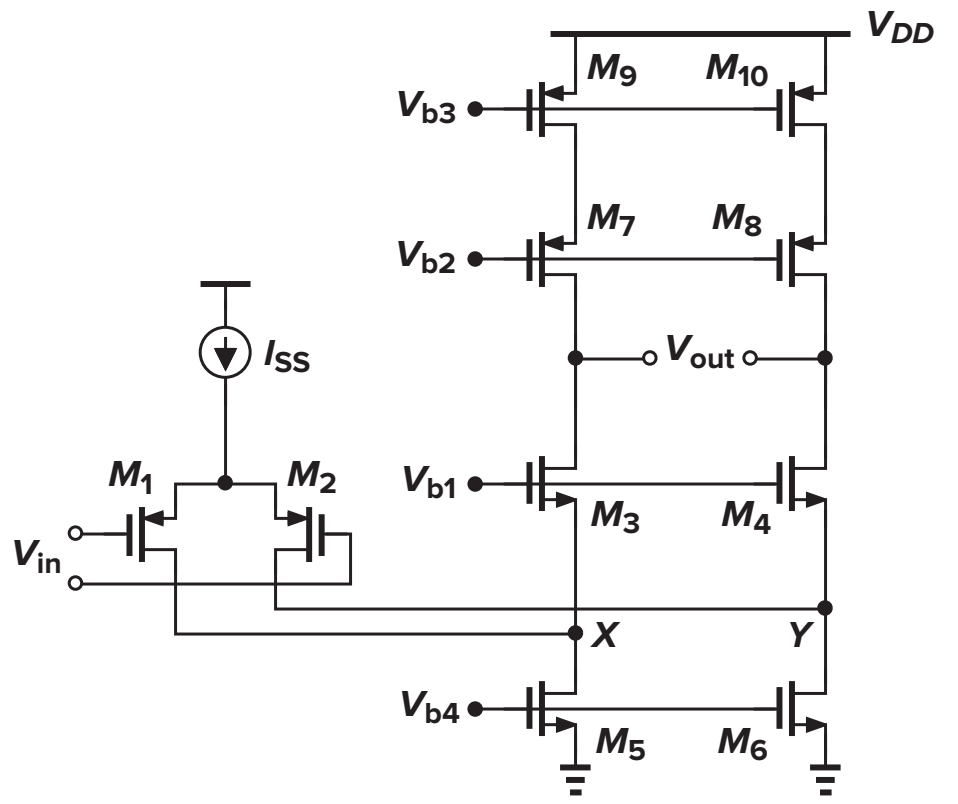
\includegraphics[width=0.40\linewidth]{../fig/ch9/fig9_15.png}\\[0.1em]{\small\sffamily 圖 9.15\quad Folded-cascode op amp（p.357）}\end{center}
\begin{center}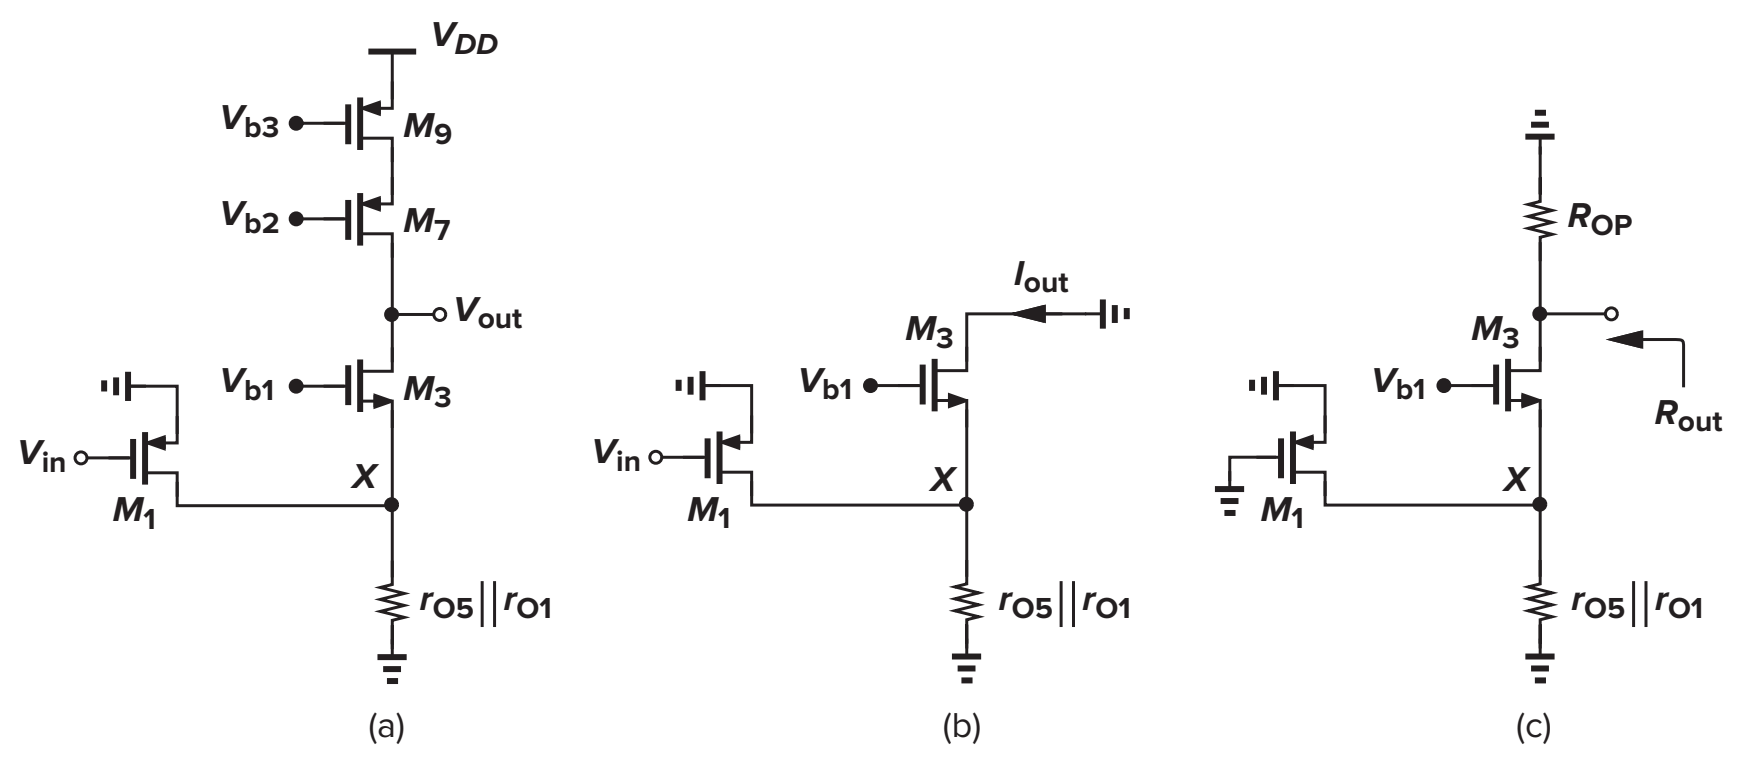
\includegraphics[width=0.80\linewidth]{../fig/ch9/fig9_16.png}\\[0.1em]{\small\sffamily 圖 9.16\quad (a) 半電路、(b) 求 $G_m$、(c) 求 $R_{out}$（p.357）}\end{center}
\begin{enumerate}[leftmargin=2.2em]
  \item \textbf{取半電路，寫成 $|A_v|=G_mR_{out}$}。
  \item \textbf{求 $G_m$（輸出短路）}：$M_1$ 的汲極電流在節點 $X$ 分給「往 $M_3$ 源極看進去的阻抗」$(g_{m3}+g_{mb3})^{-1}\pl r_{O3}$ 與 $r_{O1}\pl r_{O5}$。前者遠小於後者，故電流幾乎全進 $M_3$：
  \[G_m\approx g_{m1}\]
  \item \textbf{求 $R_{out}$}：往上看是 PMOS cascode $R_{OP}\approx(g_{m7}+g_{mb7})r_{O7}r_{O9}$；往下看是 $M_3$ 以 $r_{O1}\pl r_{O5}$ 為退化電阻的 cascode：$(g_{m3}+g_{mb3})r_{O3}(r_{O1}\pl r_{O5})$。兩者並聯：
  \[
  \boxed{|A_v|\approx g_{m1}\Big\{\big[(g_{m3}+g_{mb3})r_{O3}(r_{O1}\pl r_{O5})\big]\pl\big[(g_{m7}+g_{mb7})r_{O7}r_{O9}\big]\Big\}}
  \]
  \item \textbf{與 telescopic 比較}：PMOS 輸入對的 $g_m$ 較低；$r_{O1}$ 與 $r_{O5}$ 並聯（$M_5$ 要扛輸入管加 cascode 的電流，$r_{O5}$ 更小）使 $R_{out}$ 下降。結果增益通常\textbf{低 2--3 倍}。
\end{enumerate}
\end{derivationbox}

\textbf{非主極點較低}（圖 9.17）：folding point（$M_3$ 源極）的總電容除了 $C_{GS3},C_{SB3},C_{DB1},C_{GD1}$，還多了 $C_{GD5}$、$C_{DB5}$；$M_5$ 要用小 overdrive 扛大電流，所以很寬、電容很大。
\rfig{17}{0.55}{Telescopic 與 folded-cascode 非主極點的電容（p.358）}

\textbf{NMOS 輸入 + PMOS cascode}（圖 9.18）：NMOS 遷移率高、增益可能較高，但 folding point 的極點更低——該極點約為 $(g_{m3}+g_{mb3})/C_X$，而 PMOS $M_3$ 的 $g_m$ 小、$M_5$ 要扛 $M_1$ 加 $M_3$ 的電流而很寬。對 flicker noise 敏感的應用偏好 \textbf{PMOS 輸入}。
\rfig{18}{0.62}{Folded-cascode op amp 的實現（NMOS 輸入）（p.358）}

\textbf{Folded cascode 為何仍較常用}：相對 telescopic，它的總擺幅只略大，卻付出較高功耗、較低增益、較低極點、較高雜訊；但 (1) 輸入與輸出 CM 可以相等而不限制擺幅，(2) 可容納更寬的輸入 CM 範圍。圖 9.19 的閉迴路放大器中，$M_1$、$M_2$ 閘極幾乎不動，$V_X$、$V_Y$ 可擺到距離地或 $V_{DD}$ 兩個 overdrive（對照 \exref{9.6} 的 telescopic 只有 $\pm(V_{TH}-V_{OD})$）。圖 9.18 中 $V_{in,CM}$ 需大於 $V_{GS1,2}+\OD{11}$，上限可達 $V_{b2}+|V_{GS3}|+V_{TH1,2}$，甚至可超過 $V_{DD}$；PMOS 輸入版本則可低到 0。
\rfig{19}{0.65}{(a) 回授放大器、(b)(c) 用 folded cascode 實現（p.359）}

\exhead{9.9}{359}{NMOS 輸入 folded-cascode op amp 設計（新電路）}
\rfig{20}{0.30}{輸入輸出短接的 folded-cascode（p.360）}
規格同 \exref{9.7}（課本誤植為 Example 9.5）：$V_{DD}=3$\,V、差動擺幅 3\,V、10\,mW、增益 2000。
\begin{enumerate}[leftmargin=2.2em]
  \item \textbf{分電流}：輸入對 1.5\,mA、兩支 cascode 共 1.5\,mA、三個電流鏡 330\,$\mu$A；$M_5$、$M_6$ 各 1.5\,mA。
  \item \textbf{分 overdrive}：$M_5$--$M_6$ 給 0.5\,V（避免太寬）、$M_3$--$M_4$ 給 0.4\,V、$M_7$--$M_{10}$ 給 0.3\,V。得 $(W/L)_{5,6}=400$、$(W/L)_{3,4}=313$、$(W/L)_{7\text{--}10}=278$。輸出最低 $0.6$\,V、最高 $3-0.9=2.1$\,V，最佳輸出 CM $=1.35$\,V。
  \item \textbf{輸入對}：若輸入 CM = 輸出 CM，$V_{GS1}+\OD{11}=1.35$\,V；取 $\OD{11}=0.4$\,V $\Rightarrow V_{GS1}=0.95$\,V，$\OD1=0.25$\,V，$(W/L)_{1,2}=400$。
  \item \textbf{增益}：$g_{m1,2}=6$\,mS、$g_{m3,4}=3.75$\,mS、$g_{m7,8}=2(0.75\text{m})/0.3=5$\,mS（課本誤植為 0.05\,A/V）；$r_{O1,2}=r_{O7\text{--}10}=13.3$\,k$\Omega$，$r_{O3,4}=2r_{O5,6}=6.67$\,k$\Omega$。往 $M_7$ 汲極看 $g_{m7}r_{O7}r_{O9}=0.89$\,M$\Omega$（課本因 $g_m$ 誤植寫 8.8\,M$\Omega$）；往 $M_3$ 汲極看 $g_{m3}r_{O3}(r_{O1}\pl r_{O5})=66.7$\,k$\Omega$。增益 $\approx6\text{m}\times(66.7\text{k}\pl0.89\text{M})\approx\boxed{372}$（課本「約 400」），受 $M_3$ 有限本質增益限制。
  \item \textbf{改善方向}：$r_{O5,6}\ll r_{O1,2}$，先加長 $M_5$--$M_6$；加寬 $M_1$--$M_2$ 以提高 $g_m$；把 $M_3$、$M_4$ 的 $W$、$L$ 加倍以加倍本質增益（代價是 $X$、$Y$ 電容）。同樣需要 CMFB。
\end{enumerate}

\textbf{單端輸出}（圖 9.21）：(a) 的 PMOS cascode 電流鏡讓 $V_X=V_{DD}-|V_{GS5}|-|V_{GS7}|$，$V_{out,max}=V_{DD}-|V_{GS5}|-|V_{GS7}|+|V_{TH6}|$，浪費一個 $V_{TH}$；(b) 改用低電壓 cascode 讓 $M_7$、$M_8$ 在 triode 邊緣。單端版相對差動版有兩個缺點：擺幅只有一半、$X$ 有 mirror pole。因此偏好差動拓撲（但要 CMFB）。
\rfig{21}{0.55}{單端輸出 cascode op amp（p.360）}

%=====================================================================
\section{兩級 op amp：第一級給增益、第二級給擺幅}
單級 op amp 只做一次電壓$\to$電流轉換，增益受限於 $g_m R_{out}$，而 cascode 又吃掉擺幅。兩級架構把增益與擺幅需求\textbf{分開}：第一級高增益，第二級通常是 CS 級以得到最大擺幅。
\rfig{22}{0.33}{Two-stage op amp（p.361）}
圖 9.23：兩級增益分別為 $g_{m1,2}(r_{O1,2}\pl r_{O3,4})$ 與 $g_{m5,6}(r_{O5,6}\pl r_{O7,8})$，總增益與 cascode op amp 相當，但每個輸出可擺 $V_{DD}-|\OD{5,6}|-\OD{7,8}$，是\textbf{可能的最大值}。
\rfig{23}{0.40}{Two-stage op amp 的簡單實現（p.361）}
第一級改用 cascode（圖 9.24）：第二級增益約 10 時，$X$、$Y$ 擺幅很小，$M_1$--$M_8$ 可針對增益最佳化：
\begin{align}
A_v\approx\Big\{g_{m1,2}\big[(g_{m3,4}+g_{mb3,4})r_{O3,4}r_{O1,2}\big]\pl\big[(g_{m5,6}+g_{mb5,6})r_{O5,6}r_{O7,8}\big]\Big\}\times\big[g_{m9,10}(r_{O9,10}\pl r_{O11,12})\big]
\end{align}
\rfig{24}{0.46}{第一級採用 cascode 的兩級 op amp（p.362）}
單端輸出（圖 9.25）：第一級維持差動，只用 $M_7$--$M_8$ 電流鏡把兩個輸出級的差動電流轉成單端。三級以上很少用：每級至少一個極點，回授時難以穩定（Ch.10）。
\rfig{25}{0.33}{單端輸出的兩級 op amp（p.362）}

\exhead{9.10}{363}{兩級 op amp 設計（新方法：從輸出級開始算）}
規格：$V_{DD}=1$\,V、$P=1$\,mW、差動 $1\,V_{pp}$、增益 100；參數同 \exref{9.7} 但 $V_{THN}=0.3$\,V、$V_{THP}=-0.35$\,V。
\begin{enumerate}[leftmargin=2.2em]
  \item \textbf{分電流}：$M_1$--$M_8$ 共 960\,$\mu$A，每顆 120\,$\mu$A；偏壓 40\,$\mu$A。
  \item \textbf{第一級擺幅很小}：若第二級增益 5、單端 $0.5\,V_{pp}$，$X$ 只需 $0.1\,V_{pp}$，故 $|\OD3|+\OD1+V_{I_{SS}}$ 很寬鬆。但 (1) 電流源 $M_3$、$M_4$ 的雜訊要大 overdrive 才小；(2) $M_1$、$M_2$ 需要大 $g_m$，即小 overdrive（實際上常進入 subthreshold，本例忽略）。
  \item \textbf{輸出級 overdrive 對調}：若輸出 NMOS 0.2\,V、PMOS 0.3\,V，則 $M_5$、$M_6$ 的 $g_m$ 偏低、$M_7$、$M_8$ 雜訊大；故改成 $M_7$、$M_8$ 給 0.3\,V，$M_5$、$M_6$ 給 0.2\,V（代價：$M_5$、$M_6$ 較寬、$X$、$Y$ 電容較大）。
  \item \textbf{第二級}：$g_{m5,6}=2I_D/\OD{}=(833\,\Omega)^{-1}$、$r_{O5,6}=1/(0.2\times120\mu)=41.7$\,k$\Omega$、$r_{O7,8}=83.3$\,k$\Omega$，增益 $1.2\text{m}\times27.8\text{k}\approx33$；$(W/L)_{5,6}=200$、$(W/L)_{7,8}=44$。
  \item \textbf{第一級}：$V_{DS3,4}=|V_{GS5,6}|=0.55$\,V，$M_3$、$M_4$ overdrive 若取 0.5\,V，$V_{b1}$ 只剩 0.15\,V 太低，改取 0.4\,V：$(W/L)_{3,4}=50$、$g_{m3,4}=(1.67\text{k}\Omega)^{-1}$、$r_{O3,4}=41.7$\,k$\Omega$（課本誤寫 83\,k$\Omega$，但其後增益 66 用的是 41.7\,k$\Omega$）。
  \item \textbf{輸入對}：overdrive 若取 0.5\,V，$g_{m1}/g_{m3}=4/5$，PMOS 雜訊太大；改取 0.1\,V：$g_{m1,2}=(417\,\Omega)^{-1}$、$(W/L)_{1,2}=400$，第一級增益 $g_{m1}(r_{O1}\pl r_{O3})=2.4\text{m}\times(83.3\text{k}\pl41.7\text{k})\approx66.7$。
\end{enumerate}
總增益 $\approx66.7\times33.3\approx\boxed{2200}$，遠超過 100，主因是低偏壓電流與舊製程；奈米製程的兩級 op amp 增益低很多（Ch.11）。

%=====================================================================
\section{Gain boosting：用輔助放大器把 cascode 的 $g_m$ 放大 $(A_1+1)$ 倍}

\subsection{第一種觀點：supertransistor}
電晶體前面加一個理想電壓放大器 $A_1$（圖 9.26），整體轉導為 $A_1g_m$、電壓增益 $-A_1g_mr_O$，可看成轉導 $A_1g_m$、輸出電阻 $r_O$ 的「supertransistor」。（本節忽略 body effect。）
\rfig{26}{0.65}{(a) 電晶體前接電壓放大器、(b) 等效電路（p.364）}

\begin{derivationbox}[完整推導：gain-boosted 退化級的 $G_m$ 與 $R_{out}$（式 9.19、9.21）]
\begin{center}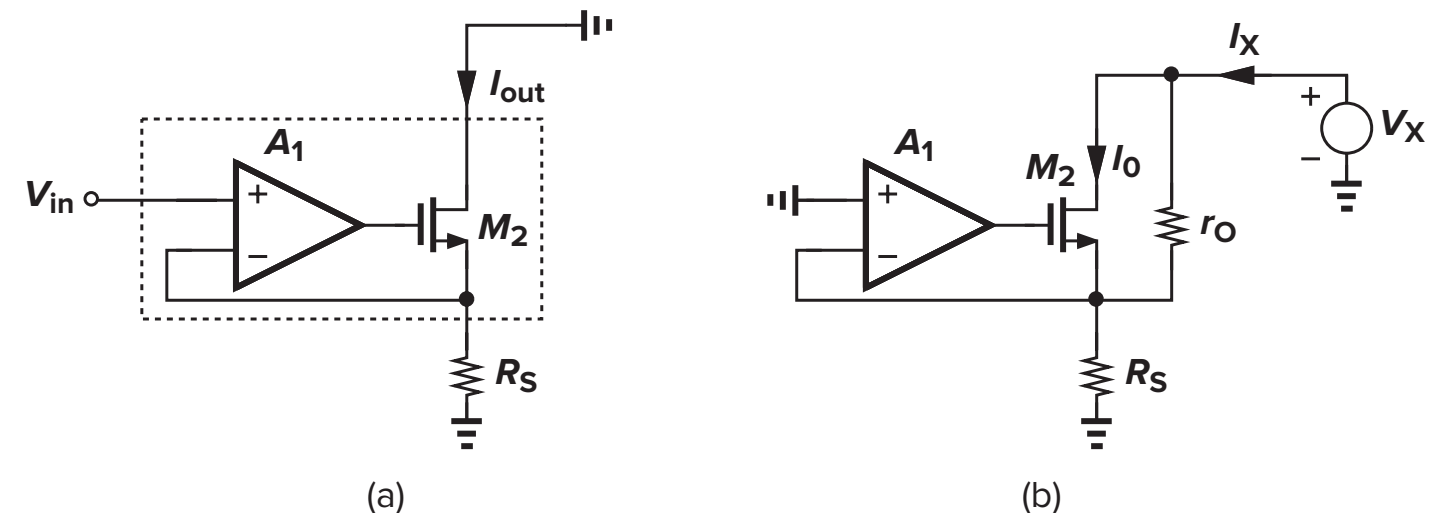
\includegraphics[width=0.55\linewidth]{../fig/ch9/fig9_27.png}\\[0.1em]{\small\sffamily 圖 9.27\quad 求 (a) 轉導、(b) 輸出電阻（p.364）}\end{center}
\begin{enumerate}[leftmargin=2.2em]
  \item \textbf{轉導（輸出接交流地）}：$R_S$ 流 $I_{out}$，閘極電壓 $(V_{in}-R_SI_{out})A_1$，$V_{GS}=(V_{in}-R_SI_{out})A_1-R_SI_{out}$，故 $I_{out}=g_m[(V_{in}-R_SI_{out})A_1-R_SI_{out}]$：
  \[\boxed{\frac{I_{out}}{V_{in}}=\frac{A_1g_m}{1+(A_1+1)g_mR_S}}\]
  沒有 $A_1$ 時為 $g_m/(1+g_mR_S)$；分子乘 $A_1$、分母是 $A_1+1$，所以 supertransistor 模型並不精確，但 $A_1\gg1$ 時誤差可忽略。
  \item \textbf{輸出電阻}：測試電流 $I_X$，$R_S$ 壓降 $I_XR_S$，閘極電壓 $-A_1I_XR_S$，故本質電流 $I_0=(-A_1R_SI_X-R_SI_X)g_m$；$r_O$ 的電流為 $(V_X-R_SI_X)/r_O$。KCL：
  \[I_X=-(A_1+1)R_Sg_mI_X+\frac{V_X-R_SI_X}{r_O}\]
  \[\Rightarrow\ \boxed{R_{out}=r_O+(A_1+1)g_mr_OR_S+R_S}\]
  沒有 $A_1$ 時為 $r_O+g_mr_OR_S+R_S$，等於把 $g_m$ 放大 $(A_1+1)$ 倍，而\textbf{汲極擺幅幾乎與普通退化電晶體相同}。
  \item \textbf{加上輸入管}（圖 9.29，把 $R_S$ 換成 $M_1$）：$R_{out}=r_{O2}+(A_1+1)g_{m2}r_{O2}r_{O1}+r_{O1}$；往 $M_2$ 源極看進去 $\approx[(A_1+1)g_{m2}]^{-1}\ll r_{O1}$，故 $G_m\approx g_{m1}$：
  \[\boxed{|A_v|\approx g_{m1}g_{m2}r_{O1}r_{O2}(A_1+1)}\]
\end{enumerate}
\end{derivationbox}

\exhead{9.11}{365}{從 $M_2$ 源極看進去的電阻（$\gamma=0$）}
\rfig{28}{0.55}{(a) 電路、(b) 測試電路（p.365）}
閘極電壓 $-A_1V_X$，$I_0=(-A_1V_X-V_X)g_m$；$R_D$ 流 $I_X$，汲極電壓 $I_XR_D$，$r_O$ 向下電流 $(I_XR_D-V_X)/r_O$。源極 KCL：
\begin{align}
\frac{I_XR_D-V_X}{r_O}-(A_1+1)g_mV_X+I_X=0
\ \Rightarrow\ \boxed{R_X=\frac{R_D+r_O}{1+(A_1+1)g_mr_O}}
\end{align}
沒有 $A_1$ 時為 $(R_D+r_O)/(1+g_mr_O)$，同樣是 $g_m$ 被放大 $(A_1+1)$ 倍。
\rfig{29}{0.25}{基本 gain-boosted 級（p.366）}

\subsection{第二種觀點：regulated cascode（把源極電壓釘住）}
退化級（圖 9.30a）中，汲極變化 $\Delta V$ 會讓源極變化 $\Delta V_S=\Delta V\,R_S/[r_O+(1+g_mr_O)R_S]$，可粗看成 $R_S$ 與 $g_mr_OR_S$ 的分壓。若要讓汲極電流不變需同時滿足：(a) $R_S$ 的跨壓不變、(b) 流過 $R_S$ 的電流等於汲極電流（只在 $P$ 接定電壓源只能滿足 (a)）。做法：用放大器比較 $V_P$ 與 $V_b$，把誤差 $A_1(V_b-V_P)$ 送回 $M_2$ 閘極（圖 9.30b）。汲極上升 $\to V_P$ 想上升 $\to$ 閘極下降 $\to$ 電流減少；效果相當於 $R_S$ 與 $A_1g_mr_OR_S$ 分壓。$A_1\to\infty$ 時 $V_P$ 被釘在 $V_b$，汲極電流恰為 $V_b/R_S$。
\rfig{30}{0.80}{(a) 退化 CS 級、(b) gain-boosted 級對輸出變化的響應（p.366）}

\exhead{9.12}{367}{Regulated cascode 內部的小訊號電壓與電流（重要新觀察）}
\rfig{31}{0.32}{Regulated cascode 的輸出阻抗測試（p.367）}
設 $(A_1+1)g_mr_OR_S$ 很大。由 \exref{9.11} 前的分析 $V_X=[r_O+(A_1+1)g_mr_OR_S+R_S]I_X$，$V_P=I_XR_S$：
\begin{align}
V_P&=\frac{R_S}{r_O+(A_1+1)g_mr_OR_S+R_S}V_X\approx\frac{V_X}{(A_1+1)g_mr_O},\\
V_G&=-A_1V_P=\frac{-A_1R_S}{r_O+(A_1+1)g_mr_OR_S+R_S}V_X,\\
V_{GS}&=V_G-V_P\approx-\frac{V_X}{g_mr_O}\ \Rightarrow\ I_0\approx-\frac{V_X}{r_O},\qquad
I_{ro}=\frac{V_X-V_P}{r_O}\approx\frac{V_X}{r_O}.
\end{align}
\textbf{觀察}：放大器把 $R_S$ 上的變化再壓小 $(A_1+1)$ 倍；$I_0$ 與 $I_{ro}$ 幾乎大小相等、方向相反——放大器調整閘極讓本質電流抵銷 $r_O$ 的電流，小訊號電流在 $r_O$ 內部「循環」，因此幾乎不流出汲極。

\subsection{電路實現}
\textbf{(a) NMOS CS 級當 $A_1$}（圖 9.32a）：$|A_1|=g_{m3}r_{O3}$，增益 $\approx g_{m1}r_{O1}g_{m2}r_{O2}(g_{m3}r_{O3}+1)$，像 triple cascode；但 $V_P$ 最低是 $V_{GS3}$，$V_{out}$ 必須高於 $V_{GS3}+(V_{GS2}-V_{TH2})$，擺幅受限。\\
\textbf{(b) PMOS CS 級}：$V_P$ 可低到 $M_1$ 的 overdrive，但若 $V_P=V_{GS1}-V_{TH1}$，$V_G=V_{GS2}+V_{GS1}-V_{TH1}$，$M_3$ 的汲極比閘極高 $V_{GS2}$，當 $V_{GS2}>|V_{TH3}|$ 時 $M_3$ 落入 triode。\\
\textbf{(c) 插入 NMOS CG 級}（即 folded cascode）：$M_4$ 由源極到汲極做向上的位準平移，讓 $V_G$ 可高於 $M_3$ 汲極。
\rfig{32}{0.48}{Gain-boosted 放大器：(a) NMOS CS、(b) PMOS CS、(c) folded cascode 輔助放大器（p.368）}

\exhead{9.13}{369}{圖 9.32(c) 中 $V_b$ 的允許範圍}
最小值讓 $I_1$ 在 triode 邊緣：$V_{b,min}=V_{GS4}+V_{I1}$；最大值讓 $M_4$ 在 triode 邊緣：$V_{b,max}=V_{GS2}+V_P+V_{TH4}$。範圍相當寬，$V_b$ 不必精確。

\textbf{差動 cascode 的 gain boosting}（圖 9.33）：$X$、$Y$ 是差動訊號，兩個單端 $A_1$、$A_2$ 可合併成一個差動放大器。(c) 用 NMOS 差動對實現時，$M_3$ 汲極最低為 $\OD3+V_{GS5}+V_{I_{SS2}}$，比普通差動 cascode 高約一個 $V_{TH}$。改用 \textbf{PMOS 輸入 folded cascode} 當輔助放大器（圖 9.34），$X$、$Y$ 最低只需 $\OD{1,2}+V_{I_{SS1}}$。
\rfig{33}{0.75}{差動 cascode 的輸出阻抗提升（p.369）}
\rfig{34}{0.45}{Folded cascode 當輔助放大器（p.370）}

\exhead{9.14}{370}{圖 9.34 的輸出阻抗}
\rfig{35}{0.30}{半電路等效（p.370）}
半電路中，$X$ 到 $P$ 的增益 $\approx g_{m5}R_{out1}$，$R_{out1}\approx[g_{m7}r_{O7}(r_{O9}\pl r_{O5})]\pl(g_{m11}r_{O11}r_{O13})$，故
\[
R_{out}\approx g_{m3}r_{O3}r_{O1}\cdot g_{m5}R_{out1},
\]
相當於「四重 cascode」。PMOS 負載也可用 regulated cascode（圖 9.36），$A_2$ 要用 NMOS 輸入 folded cascode 才不限制擺幅。
\rfig{36}{0.65}{訊號路徑與負載同時 gain boosting（p.371）}

\subsection{頻率響應：多一個 pole--zero，第二極點約在 $A_0\omega_0$ 之上}
Gain-boosted op amp 仍算「單級」：大部分訊號直接經 cascode 到輸出，只有小「誤差」分量經過（並被延遲於）輔助放大器。分析圖 9.37，$A_1(s)=A_0/(1+s/\omega_0)$，只計 $C_L$。
\rfig{37}{0.33}{頻率響應分析電路（p.371）}
由 \exref{9.11}，往 $M_2$ 源極看進去為 $r_{O2}/[1+(A_1+1)g_{m2}r_{O2}]$，與 $r_{O1}$ 分流：
\begin{align}
G_m(s)&=g_{m1}\frac{r_{O1}}{r_{O1}+\frac{r_{O2}}{1+(A_1+1)g_{m2}r_{O2}}}
=\frac{g_{m1}r_{O1}[1+(A_1+1)g_{m2}r_{O2}]}{r_{O1}+(A_1+1)g_{m2}r_{O2}r_{O1}+r_{O2}},\\
Z_{out}&=[r_{O1}+(A_1+1)g_{m2}r_{O2}r_{O1}+r_{O2}]\pl\frac{1}{C_Ls},\\
\frac{V_{out}}{V_{in}}&=-G_mZ_{out}=\frac{-g_{m1}r_{O1}[1+(A_1+1)g_{m2}r_{O2}]}{(r_{O1}+r_{O2})C_Ls+(A_1+1)g_{m2}r_{O2}r_{O1}C_Ls+1}.
\end{align}
\textbf{注意}：$A_1$ 在高頻會下降，不能先假設 $A_1\gg1$ 而丟項。代入 $A_1(s)$ 得到二階轉移函數（式 9.39），結果：
\begin{align}
|\omega_z|&\approx(A_0+1)\omega_0\quad(\text{左半平面零點，約為輔助放大器的 GBW})\\
|\omega_{p1}|&=\frac{1}{[r_{O1}+(A_0+1)g_{m2}r_{O2}r_{O1}+r_{O2}]C_L+1/\omega_0}\approx\frac{1}{A_0g_{m2}r_{O2}r_{O1}C_L}\\
|\omega_{p2}|&\approx(A_0+1)\omega_0+\frac{1}{g_{m2}r_{O2}r_{O1}C_L}
\end{align}
第二極點約在原 cascode 的 $-3$\,dB 頻寬 $(g_{m2}r_{O2}r_{O1}C_L)^{-1}$ 之上再加 $A_0\omega_0$。

\exhead{9.15}{373}{主極點近似是否成立？}
設 $(A_0+1)g_{m2}r_{O2}r_{O1}\gg r_{O1},r_{O2}$：
\[
\frac{\omega_{p2}}{\omega_{p1}}\approx(A_0+1)^2g_{m2}r_{O2}r_{O1}C_L\omega_0+2(A_0+1)+\frac{1}{g_{m2}r_{O2}r_{O1}C_L\omega_0},
\]
第二項 $2(A_0+1)$ 就遠大於 1，故近似成立。
\rfig{38}{0.48}{Gain-boosted 級的頻率響應（p.373）}
%=====================================================================
\section{四種拓撲比較與輸出擺幅的驗證方法}

課本 Table 9.1（p.374）：

\begin{center}
\begin{tabular}{lccccc}
\toprule
 & Gain & Output Swing & Speed & Power & Noise\\\midrule
Telescopic & Medium & Medium & Highest & Low & Low\\
Folded-Cascode & Medium & Medium & High & Medium & Medium\\
Two-Stage & High & Highest & Low & Medium & Low\\
Gain-Boosted & High & Medium & Medium & High & Medium\\
\bottomrule
\end{tabular}
\end{center}

\textbf{輸出擺幅怎麼驗證}：奈米元件的飽和／triode 邊界模糊，不能只看工作區。做法是輸入逐漸變大的正弦波，監看 $|V_{out}/V_{in}|$，增益開始下降（例如掉 10\%，約 1\,dB）時的輸出幅度 $V_1$ 即最大「允許」擺幅；若關心失真，就把 op amp 放進實際閉迴路（如反相放大器），量輸出諧波，取可接受失真下的最大幅度（p.374）。

%=====================================================================
\section{Common-mode feedback：高增益全差動電路一定要 CMFB}

\subsection{為什麼需要：差動回授定不了 CM}
電阻負載差動對把輸入輸出短接（圖 9.40b），CM 位準 $V_{DD}-I_{SS}R_D/2$ 定義得很清楚。但換成 PMOS 電流源負載（圖 9.41）以提高增益後，輸出 CM 取決於 $I_{D3,4}$ 與 $I_{SS}/2$ 有多接近：若 $I_{D3,4}$ 略大於 $I_{SS}/2$，$M_3$、$M_4$ 必須進 triode 才能讓電流降到 $I_{SS}/2$；反之 $V_X$、$V_Y$ 要下降到 $M_5$ 進 triode。
\rfig{40}{0.50}{(a) 電阻負載差動對、(b) 輸入輸出短接（p.375）}
\rfig{41}{0.58}{(a) 高增益差動對短接、(b) 電流鏡失配的影響（p.375）}
本質原因（圖 9.42）：p 型電流源要和 n 型電流源平衡，差額 $I_P-I_N$ 流過放大器的本質輸出阻抗，造成 $(I_P-I_N)(R_P\pl R_N)$ 的電壓誤差；$R_P\pl R_N$ 很大，所以小失配就把某一側推進 triode。\textbf{經驗法則}：若輸出 CM 不能「目視」決定、需要依元件參數計算，它就是定義不良的。
\rfig{42}{0.16}{高增益放大器的簡化模型（p.376）}

\begin{trapbox}[常見陷阱：CMFB 的兩個典型錯誤]
\begin{enumerate}[leftmargin=2.2em]
  \item \textbf{以為差動回授會修正輸出 CM}：從 $X$、$Y$ 回到輸入的差動回授無法阻止輸出 CM 往 $V_{DD}$ 或地漂走。
  \item \textbf{模擬時微調 $V_b$ 讓 $V_X$、$V_Y\approx V_{DD}/2$，就說不需要 CMFB}：真實電路一定有上下電流源的隨機失配，CM 會大幅漂移，沒有 CMFB 的 op amp 會失效。
\end{enumerate}
\end{trapbox}

\exhead{9.16}{376}{1\% 尾電流失配的後果（重要新觀察）}
\rfig{43}{0.36}{\exref{9.7} 的 telescopic op amp 加偏壓電流鏡（p.376）}
\exref{9.7}（課本誤寫 Example 9.5）的單端輸出阻抗為 266\,k$\Omega$（PMOS 加長後 $667\text{k}\pl444\text{k}$）。$M_9$ 失配使 $I_{SS}=2.97$\,mA，$M_3$ 與 $M_5$ 的電流差 $30\,\mu\text{A}/2=15\,\mu$A，對應電壓誤差 $266\text{k}\times15\,\mu\text{A}=\boxed{3.99\text{ V}}$——不可能產生，於是 $V_X$、$V_Y$ 上升到 $M_5$--$M_8$ 進入 triode，使 $I_{D7,8}=1.485$\,mA。另一個 CM 誤差來源是 $I_{D7,8}$ 與 $I_{D11}$（以及 $I_{D9}$ 與 $I_{D10}$）因 $V_{DS}$ 不同造成的確定性誤差，可用 Ch.5 的電流鏡技巧降低。

CMFB 依 Ch.8 的回授觀點分三步：\textbf{感測輸出 CM}、\textbf{與參考電壓比較}、\textbf{把誤差送回偏壓網路}（圖 9.44）。
\rfig{44}{0.32}{CMFB 概念架構（p.377）}

\subsection{CM 感測方法}
\begin{tabularx}{\linewidth}{>{\raggedright}p{3.0cm}>{\raggedright}p{4.6cm}X}
\toprule
方法 & 原理 & 缺點 \tabularnewline\midrule
電阻分壓（圖 9.45） & $V_{out,CM}=\dfrac{R_1V_{out2}+R_2V_{out1}}{R_1+R_2}$，$R_1=R_2$ 時為平均值 & $R_1,R_2$ 必須遠大於 op amp 輸出阻抗（如 266\,k$\Omega$ 需數 M$\Omega$），面積大、寄生電容大。 \tabularnewline
源極隨耦器 + 電阻（圖 9.46） & 消除電阻負載；感測到的 CM 低 $V_{GS7,8}$，比較時補償即可 & (1) 大差動擺幅時隨耦器會被「餓死」：$I_1$ 要同時吸 $I_X\approx(V_{out2}-V_{out1})/(R_1+R_2)$ 與 $I_{D7}$；(2) $V_{out1,min}=V_{GS7}+V_{I1}$（約兩個 overdrive 加一個 $V_{TH}$），每邊擺幅少約 $V_{TH}$。 \tabularnewline
深 triode MOS（圖 9.48） & $R_{tot}=R_{on7}\pl R_{on8}$ $=1/[\mu_nC_{ox}\frac WL(V_{out1}+V_{out2}-2V_{TH})]$，只與和有關 & 擺幅受限：某輸出降到約 $V_{TH}$ 時對應的管子進入飽和，$R_{on}$ 變化不再互相抵消。 \tabularnewline
差動對比較 $V_{REF}$（圖 9.50） & 小訊號 $I_{CM}\propto V_{out1}+V_{out2}$ & 大擺幅時差動對非線性，$f(V_{out1}-V_{REF})+f(V_{out2}-V_{REF})$ 依個別值而定，重建的 CM 會隨差動訊號變動。 \tabularnewline
電容感測 & 不降低低頻增益 & 在 Ch.13 討論。 \tabularnewline
\bottomrule
\end{tabularx}

\rfig{45}{0.30}{電阻感測（p.377）}
\rfig{46}{0.45}{用源極隨耦器感測（p.378）}
\rfig{47}{0.36}{大擺幅時源極隨耦器電流被餓死（p.378）}
\rfig{48}{0.55}{(a) 深 triode MOS 感測、(b) 使 $M_7$ 達飽和邊緣的輸出位準（p.379）}
CM 感測的核心要求：\textbf{產生的量必須與差動訊號無關}。

\exhead{9.17}{379}{步級響應中兩輸出不對稱}
\rfig{49}{0.22}{模擬波形（p.379）}
從 $t_1$ 到 $t_2$ 輸出 CM 改變了，表示 CM 感測非線性、把兩個時刻的 CM 解讀成不同值。例如 $M_7$ 或 $M_8$ 在 $t_2$ 不再處於深 triode，式 (9.49) 不成立，$V_{CM}$ 成為差動訊號的函數。
\rfig{50}{0.45}{高度非線性的 CM 感測電路（p.380）}

\subsection{CM 回授方法}
\textbf{誤差放大器控制電流源}（圖 9.51）：$V_{out1}$、$V_{out2}$ 一起上升 $\to V_E$ 上升 $\to M_3$、$M_4$ 電流增加 $\to$ 輸出 CM 下降；loop gain 大時輸出 CM 趨近 $V_{REF}$。也可回授到 PMOS 電流源，或只控制部分電流（把 $M_3$ 拆成定電流與受控兩顆並聯），以最佳化 settling。Folded cascode 中可控制輸入對的尾電流（圖 9.52）：輸出上升 $\to$ 尾電流增加 $\to M_5$--$M_6$ 流入 cascode 的電流減少 $\to$ 輸出回降。
\rfig{51}{0.48}{感測並控制輸出 CM（p.380）}
\rfig{52}{0.48}{另一種控制輸出 CM 的方法（p.381）}

\textbf{Triode 感測直接當回授}（圖 9.53）：$R_{on7}\pl R_{on8}$ 調整 $M_5$、$M_6$ 的偏壓電流，使 $I_{D5,6}$ 恰等於 $I_{D9,10}=I_D$：$V_b-V_{GS5}=2I_D(R_{on7}\pl R_{on8})$，代入式 (9.49)：
\begin{align}
V_{out1}+V_{out2}=\frac{2I_D}{\mu_nC_{ox}(W/L)_{7,8}}\cdot\frac{1}{V_b-V_{GS5}}+2V_{TH},\qquad V_{GS5}=\sqrt{\frac{2I_D}{\mu_nC_{ox}(W/L)_5}}+V_{TH5}.
\end{align}
缺點：(1) 輸出 CM 是元件參數的函數；(2) $R_{on7}\pl R_{on8}$ 的壓降限制擺幅；(3) 為減少壓降 $M_7$、$M_8$ 很寬，輸出電容大。把回授改到輸入對尾電流（圖 9.54）可緩解 (2)。
\rfig{53}{0.26}{用 triode 元件的 CMFB（p.381）}
\rfig{54}{0.42}{控制輸出 CM 的另一種方法（p.382）}

\exhead{9.18}{382}{輸出 CM 對 $V_b$ 的靈敏度（重要新觀察）}
\rfig{55}{0.38}{簡化的 CMFB 迴路（p.383）}
令 $V_{in}=0$，在 $M_7$、$M_8$ 閘極斷開迴路。triode 區 $g_{m7}=g_{m8}=\mu_nC_{ox}(W/L)_{7,8}V_{DS7,8}$（$V_{DS7,8}$ 通常 $<100$\,mV）。loop gain 夠大時閉迴路增益 $\approx1/\beta$：
\begin{align}
\beta&=\frac{V_2}{V_1}\Big|_{I_2=0}=-(g_{m7}+g_{m8})(R_{on7}\pl R_{on8})\nonumber\\
&=-2\mu_nC_{ox}\Big(\frac WL\Big)_{7,8}V_{DS7,8}\cdot\frac{1}{2\mu_nC_{ox}(W/L)_{7,8}(V_{GS7,8}-V_{TH7,8})}\nonumber\\
&=-\frac{V_{DS7,8}}{V_{GS7,8}-V_{TH7,8}}
\qquad\Rightarrow\qquad
\boxed{\left|\frac{dV_{out,CM}}{dV_b}\right|_{closed}\approx\frac{V_{GS7,8}-V_{TH7,8}}{V_{DS7,8}}}
\end{align}
$V_{GS7,8}$（即輸出 CM）約 $V_{DD}/2$，所以靈敏度可能遠大於 1；要降低就要加大 $V_{DS7,8}$，但會犧牲 loop gain。

\textbf{改良：用電流鏡定義 $V_b$}（圖 9.56）：取 $(W/L)_{15}=(W/L)_9$、$(W/L)_{16}=(W/L)_7+(W/L)_8$，則只有 $V_{out,CM}=V_{REF}$ 時 $I_{D9}=I_1$，輸出 CM 等於參考值且不需電阻感測。$V_{DS15}\ne V_{DS9}$ 造成的通道長度調變誤差，可再用 $M_{17}$、$M_{18}$ 複製 $M_1$、$M_2$ 源極電壓來消除（圖 9.57）。
\rfig{56}{0.48}{(a) 更精確定義輸出 CM 的 CMFB 修改（p.384）}

\textbf{電阻式 CMFB}（圖 9.58b）：對差動訊號 $P$ 為虛地，增益 $g_{m1,2}(r_{O1,2}\pl r_{O3,4}\pl R_F)$，宜取 $R_F\gg r_{O1,2}\pl r_{O3,4}$；對 CM，$M_3$、$M_4$ 是二極體接法，CM 位準 $V_{DD}-|V_{GS3,4}|$ 定義清楚。適用低增益應用。(c) 從電阻抽小電流 $I_1$，使汲極比 $V_P$ 高 $I_1R_F/2$；若 $I_1R_F/2=|V_{TH3,4}|$，PMOS 在飽和邊緣，最小 $V_{DD}$ 降為三個 overdrive。
\rfig{58}{0.65}{(a) 二極體負載差動對、(b) 電阻式 CMFB、(c) 低電壓修改（p.385）}

\exhead{9.19}{385}{圖 9.58(b) 的最大擺幅}
下限：選 $V_{in,CM}$ 讓 $I_{SS}$ 在 triode 邊緣，每個輸出可降到地上兩個 overdrive。上限：輸出 CM 加 $|V_{TH3,4}|$，即 $V_{DD}-|V_{GS3,4}|+|V_{TH3,4}|=V_{DD}-|V_{GS3,4}-V_{TH3,4}|$。

\exhead{9.20}{385}{用兩顆 triode 元件取代尾電流源（新電路，觀察 CMRR 很差）}
\rfig{59}{0.68}{(a) 學生的電路、(b) 輸出短接、(c) 小訊號等效（p.385）}
電路對稱時輸出可短接成 (b)。複合電晶體 $M_5+M_6$：$g_{m,tail}=2\mu_nC_{ox}(W/L)_{5,6}V_P$，通道電阻 $R_{tail}=[2\mu_nC_{ox}(W/L)_{5,6}(V_{out,CM}-V_{TH5,6})]^{-1}$。設 $M_1$、$M_2$ 的 $\lambda=\gamma=0$：$M_1+M_2$ 的小訊號電流為 $-V_{out,CM}/(r_{O3,4}/2)$，對應 $V_{GS}=-V_{out}/(g_{m1,2}r_{O3,4})$，故 $V_P=V_{in,CM}+V_{out}/(g_{m1,2}r_{O3,4})$，流過 $R_{tail}$ 的電流加上 $g_{m,tail}V_{out,CM}$ 必須等於 $-V_{out,CM}/(r_{O3,4}/2)$：
\[
\frac{V_{out,CM}}{V_{in,CM}}=\boxed{-\frac{1}{\dfrac{2R_{tail}}{r_{O3,4}}+g_{m,tail}R_{tail}+(g_{m1,2}r_{O3,4})^{-1}}}
\]
三項都小於 1（$R_{tail}$ 很小、$g_{m,tail}R_{tail}=V_P/(V_{out,CM}-V_{TH})<1$、$g_mr_O\gg1$），所以 CM 增益約為 1：輸入 CM 誤差幾乎不衰減地到輸出，CMRR 很差。

\subsection{兩級 op amp 的 CMFB}
圖 9.60 比較三種做法：
\begin{itemize}[leftmargin=1.5em]
  \item \textbf{(b) 只控制第二級 $V_{b2}$}：第一級 $X$、$Y$ 的 CM 沒人管。若 $I_{SS}$ 小於 $M_3+M_4$ 想抽的電流，$V_X$、$V_Y$ 上升把它們推進 triode，$|V_{GS5,6}|$ 也跟著減小，$M_5$--$M_8$ 電流遠低於設計值。\textbf{不可用}。
  \item \textbf{(c) 感測輸出 CM、回授到第一級 $I_{SS}$}：輸出太高 $\to$ 減小 $I_{SS}$ $\to V_X,V_Y$ 上升 $\to |I_{D5,6}|$ 下降 $\to$ 輸出下降；$M_5$、$M_6$ 實際上在感測 $X$、$Y$ 的 CM，所以一個迴路管兩級（若 $M_3$、$M_4$ 有自己的尾電流就失效）。但迴路有 $X$、主輸出、誤差放大器、以及大 $R_{CM}$ 與 $A_e$ 輸入電容各一個極點，共 3--4 個，\textbf{難以穩定}（圖 9.61）。
  \item \textbf{兩個獨立迴路}（圖 9.62）：$R_1$、$R_2$ 管第一級、$R_3$、$R_4$ 管第二級，所有電流都由 $I_{SS}$ 複製：$R_1,R_2$ 調 $V_{GS3,4}$ 直到 $|I_{D3}|=|I_{D4}|=I_{SS}/2$；$V_{GS3,4}=V_{GS5,6}$ 讓 $M_5$、$M_6$ 像電流鏡；$R_3,R_4$ 調 $V_{GS7,8}$ 直到 $I_{D7,8}=|I_{D5,6}|$。差動增益 $g_{m1}(r_{O1}\pl r_{O3}\pl R_1)\,g_{m5}(r_{O5}\pl r_{O7}\pl R_3)$。
\end{itemize}
\rfig{60}{0.58}{(a) 兩級 op amp、(b) 只在第二級做 CMFB、(c) 由第二級回授到第一級（p.387）}
\rfig{61}{0.42}{求 CMFB 迴路極點數的等效電路（p.387）}
\rfig{62}{0.34}{每一級各自的簡單 CMFB 迴路（p.388）}

\exhead{9.21}{388}{圖 9.62 的輸出 CM 為何偏低，如何解決}
沒有訊號時 $R_3$、$R_4$ 不流電流，輸出 CM 就等於 $V_{G7,8}$；$M_7$、$M_8$ 為了小 overdrive 而很寬，$V_{GS7,8}$ 只比 $V_{TH}$ 大一點，遠低於 $V_{DD}/2$，擺幅受限。\textbf{解法}：從節點 $Q$ 抽小電流 $I_Q$（圖 9.63），$R_3$、$R_4$ 產生 $R_3I_Q/2$ 的壓降，輸出 CM 上移同樣的量，選 $I_Q$ 使其約為 $V_{DD}/2$。
\rfig{63}{0.34}{抽電流 $I_Q$ 抬高輸出 CM（p.388）}
第一級若是 telescopic cascode（圖 9.64），在 cascode 管上做 CM 感測可避免負載高阻抗節點 $X$、$Y$，維持高增益（雖不精確）。
\rfig{64}{0.42}{在 cascode 與輸出級周圍的 CMFB 迴路（p.389）}

%=====================================================================
\section{輸入範圍限制：NMOS 與 PMOS 輸入對並聯}
在單位增益 buffer（圖 9.65）中輸入擺幅約等於輸出擺幅，擺幅反而受\textbf{輸入差動對}限制：$V_{in,min}\approx V_{out,min}=V_{GS1,2}+V_{I_{SS}}$，比 $M_5$--$M_8$ 允許的最小值高約一個 $V_{TH}$。輸入再低，尾電流源進 triode，偏壓電流與 $g_m$ 下降。
\rfig{65}{0.62}{Unity-gain buffer（p.389）}
解法：把 NMOS 與 PMOS 輸入的 folded cascode 合併（圖 9.66），一對「死掉」時另一對還「活著」：輸入 CM 接近地時 NMOS 對 $g_m\to0$ 但 PMOS 對正常；接近 $V_{DD}$ 時反之。\textbf{注意}：總轉導 $G_{m,tot}$ 隨輸入 CM 變化（圖 9.67），增益、速度、雜訊都跟著變。
\rfig{66}{0.42}{擴展輸入 CM 範圍（p.390）}
\rfig{67}{0.30}{等效轉導隨輸入 CM 的變化（p.390）}
%=====================================================================
\section{Slew rate：大訊號時充放電電流是固定的}

\subsection{線性系統的斜率正比於終值}
RC 電路對高度 $V_0$ 的步級：$\dfrac{dV_{out}}{dt}=\dfrac{V_0}{\tau}e^{-t/\tau}$，輸入加倍則每一點的輸出（與斜率）都加倍。線性 op amp 的回授電路（圖 9.69）也一樣，設 $R_1+R_2\gg R_{out}$：
\begin{align}
\frac{V_{out}}{V_{in}}(s)\approx\frac{A\big/\big(1+A\frac{R_2}{R_1+R_2}\big)}{1+\dfrac{R_{out}C_L}{1+AR_2/(R_1+R_2)}s},
\end{align}
低頻增益與時間常數都除以 $1+AR_2/(R_1+R_2)$，步級響應為指數（\textbf{linear settling}）。實際 op amp 在大步級下輸出變成\textbf{固定斜率的 ramp}，稱為 slewing，斜率即 \textbf{slew rate}（圖 9.70）。
\rfig{70}{0.55}{Op amp 電路的 slewing（p.391）}

\subsection{起因：輸入對一邊截止，回授迴路斷開}
圖 9.71 小訊號時：$\Delta V$ 使 $I_{D1}$ 增 $g_m\Delta V/2$、$I_{D2}$ 減 $g_m\Delta V/2$，電流鏡再加一份，op amp 總共輸出 $g_m\Delta V$ 給 $C_L$；$V_{out}$ 上升使 $V_X$ 上升、差動輸入變小，電流隨之減少 $\Rightarrow$ 指數響應。
\rfig{71}{0.50}{簡單 op amp 的小訊號操作（p.392）}
$\Delta V$ 大到 $M_1$ 吃下全部 $I_{SS}$、$M_2$ 截止（圖 9.72a）：\textbf{迴路斷開}，$C_L$ 以固定電流 $I_{SS}$ 充電，斜率 $I_{SS}/C_L$（忽略 $M_4$ 通道長度調變與 $R_1+R_2$ 電流），與輸入大小無關；直到 $V_X$ 接近 $V_{in}$、$M_2$ 導通才回到線性區。下降邊同理（圖 9.72b），以約 $I_{SS}$ 放電。所以 slewing 是\textbf{非線性}現象。
\rfig{72}{0.75}{(a) 低到高、(b) 高到低轉換時的 slewing（p.392）}
Slewing 的影響：小訊號頻寬看似夠快，大訊號速度卻被可用的充放電電流限制，且輸出失真大。放大穩態正弦 $V_0\sin\omega_0t$ 時需 $\boxed{SR>V_0\omega_0}$。

\exhead{9.22}{393}{電容回授放大器的小訊號步級響應與正負 slew rate（新電路）}
\rfig{73}{0.55}{(a) 電路、(b) 模型、(c)(d) 正負 slewing（p.393）}
\textbf{(a)} 以 $A_v=g_{m1,2}(r_{O2}\pl r_{O4})$、$R_{out}=r_{O2}\pl r_{O4}$ 建模，$V_X=C_1V_{out}/(C_1+C_2)$，$V_P=(V_{in}-\frac{C_1}{C_1+C_2}V_{out})A_v$，輸出節點 KCL：
\begin{align}
\Big[\Big(V_{in}-\frac{C_1}{C_1+C_2}V_{out}\Big)A_v-V_{out}\Big]\frac{1}{R_{out}}=V_{out}\frac{C_1C_2}{C_1+C_2}s\nonumber\\
\Rightarrow\quad\frac{V_{out}}{V_{in}}=\frac{A_v\big/\big(1+A_v\frac{C_1}{C_1+C_2}\big)}{1+\dfrac{\frac{C_1C_2}{C_1+C_2}R_{out}}{1+A_v\frac{C_1}{C_1+C_2}}s}
\end{align}
低頻增益與時間常數都除以 $1+A_vC_1/(C_1+C_2)$：
\begin{gather*}
V_{out}(t)=\frac{A_v}{1+A_v\frac{C_1}{C_1+C_2}}V_0\big(1-e^{-t/\tau}\big)u(t),\\
\boxed{\tau=\frac{C_1C_2}{C_1+C_2}R_{out}\Big/\Big(1+A_v\frac{C_1}{C_1+C_2}\Big)}
\end{gather*}
\textbf{(b)} 大正步級使 $M_2$ 截止（c），大負步級使 $M_1$ 截止（d）：
\[V_{out}(t)=\pm\frac{I_{SS}}{C_1C_2/(C_1+C_2)}\,t\]
輸出看到的等效電容是 $C_1$ 與 $C_2$ \textbf{串聯}。

\textbf{Telescopic op amp 的 SR}（圖 9.74）：大差動輸入時 $M_1$ 或 $M_2$ 截止，$V_{out1}$、$V_{out2}$ 以 $\pm I_{SS}/(2C_L)$ 變化，差動輸出 $\boxed{SR=I_{SS}/C_L}$。
\rfig{74}{0.55}{Telescopic op amp 的 slewing（p.394）}

\textbf{Folded cascode（單端）}（圖 9.75）：PMOS 電流源各供 $I_P$，充放電 $C_L$ 的電流為 $I_{SS}$，$SR=I_{SS}/C_L$，只要 $I_P\ge I_{SS}$ 就與 $I_P$ 無關；實務上取 $I_P\approx I_{SS}$。若 $I_{SS}>I_P$，slewing 時 $M_3$ 截止、$V_X$ 掉到很低，$M_1$ 與尾電流源進 triode；$M_2$ 導通後 $V_X$ 要大幅回擺，settling 變慢（\textbf{overdrive recovery}，圖 9.76）。解法：加 clamp 電晶體 $M_{11}$、$M_{12}$（圖 9.77），$I_{SS}-I_P$ 改流過它們，$V_X$ 只需降到足以讓 clamp 導通；(b) 直接 clamp 到 $V_{DD}$，平衡時 $V_X$、$V_Y$ 高於 $V_{DD}-V_{THN}$，clamp 在小訊號下關閉。
\rfig{75}{0.75}{Folded-cascode op amp 的 slewing：(a) 正、(b) 負步級（p.395）}
\rfig{76}{0.35}{Slewing 後 overdrive recovery 造成長 settling（p.395）}
\rfig{77}{0.50}{限制 $X$、$Y$ 擺幅的 clamp 電路（p.396）}

\textbf{提高 SR 的取捨}：$C_L$ 固定時必須加大 $I_{SS}$；為維持擺幅所有電晶體要等比例加寬 $\Rightarrow$ 功耗與輸入電容增加。電流與寬度一起縮放時 $g_mr_O$ 與開迴路增益不變。

\exhead{9.23}{396}{何時從 slewing 進入 linear settling}
\exref{9.22} 的電路在 slewing 中 $V_X$ 上升使 $M_2$ 逐漸導通。若以 $|I_{D1}-I_{D2}|<\alpha I_{SS}$（例如 $\alpha=0.1$）視為線性，由差動對大訊號式：
\begin{align}
\alpha I_{SS}=\frac12\mu_nC_{ox}\frac WL\,\Delta V_G\sqrt{\frac{4I_{SS}}{\mu_nC_{ox}W/L}-\Delta V_G^2}
\quad\Rightarrow\quad
\Delta V_G\approx\alpha\sqrt{\frac{I_{SS}}{\mu_nC_{ox}W/L}}
\end{align}
（$\sqrt{I_{SS}/(\mu_nC_{ox}W/L)}$ 是平衡時差動對每顆的 overdrive；也可用小訊號 $\alpha I_{SS}=g_m\Delta V_G$ 得到相同結果。）$V_X$ 要升到 $V_0-\Delta V_G$，$V_{out}$ 需升 $(V_0-\Delta V_G)(1+C_2/C_1)$，以 $SR=I_{SS}/[C_1C_2/(C_1+C_2)]$ 計：
\[
\boxed{t=\frac{C_2}{I_{SS}}\Big(V_0-\alpha\sqrt{\frac{I_{SS}}{\mu_nC_{ox}W/L}}\Big)}
\]
這是粗估：$M_2$ 開始導通後充電電流已非定值；$\alpha$ 依所需線性度而定（1\% 非線性允許的 $\alpha$ 比 0.1\% 大很多）。兩級 op amp 的 slewing 留待 Ch.10。

%=====================================================================
\section{高 slew rate op amp：讓充電電流在 slewing 時自動變大}

\subsection{單級：push-pull（class-AB）}
CS 級加電流源負載 $I_0$（圖 9.78a）：$V_{in}$ 往下跳使 $M_1$ 截止時 $SR=I_0/C_L$。若要負載電流在暫態時自動增加，$V_b$ 必須跟著 $V_{in}$ 跳。把 $V_{in}$ 同時加到兩管（9.78b，互補 CS）可行但 PSRR 差。改用電流鏡控制 $M_2$（圖 9.79a）：若 $I_b$ 由另一顆 CS 管產生（b），$V_{in}$ 下降時 $I_b$ 反而減少——\textbf{極性錯誤}，需要多一次反相。差動架構中 $V_{in}^+$、$V_{in}^-$ 都有：(c) 用 $V_{in}^-$ 控制 $M_2$ 的偏壓、$V_{in}^+$ 控制 $M_4$：$V_{in}^+$ 下跳、$V_{in}^-$ 上跳時，(1) $M_5$ 少抽 $M_8$ 電流，$|I_{D4}|$ 降低；(2) $M_3$ 多抽電流、放電其負載；(3) $M_6$ 多抽 $M_7$ 電流，$|I_{D2}|$ 增加；(4) $M_1$ 少抽電流，讓 $M_2$ 對汲極電容充電。這種把負載電流源變成主動上拉的電路稱 \textbf{push-pull}（class-AB），緩和速度與平均功耗的取捨。
\rfig{79}{0.80}{(a) 電流鏡偏壓的 CS 級、(b) 極性錯誤、(c) 極性正確、(d) 加尾電流源（p.398）}
(d) 加尾電流源改善輸入 CMRR。$V_{in}^+$ 上跳、$M_1$ 與 $M_5$ 吃下全部尾電流時：$M_2$ 截止，$V_{out1}$ 以 $I_{SS1}/C_L$ 下降；$M_3$ 截止，$V_{out2}$ 以 $I_{SS2}(W_4/W_8)/C_L$ 上升（$L_4=L_8$）：
\[
SR_{diff}=\frac{I_{SS1}+I_{SS2}(W_4/W_8)}{C_L}
\]
沒有 push-pull 時只有 $I_{SS1}/C_L$。取 $W_4/W_8=5$、$I_{SS2}=I_{SS1}$：SR 變 6 倍，功耗只變 2 倍。

\exhead{9.24}{398}{Class-AB op amp 的小訊號增益}
除了主路徑，電流鏡路徑把 $M_5$、$M_6$ 的電流放大 $W_4/W_8$ 倍，也貢獻增益：
\[
|A_v|\approx g_{m1}(r_{O3}\pl r_{O4})+\frac{W_4}{W_8}g_{m5}(r_{O3}\pl r_{O4})=\Big[g_{m1}+\frac{W_4}{W_8}g_{m5}\Big](r_{O3}\pl r_{O4})
\]
等效轉導由 $g_{m1}$ 提高到 $g_{m1}+(W_4/W_8)g_{m5}$。

\textbf{Mirror pole 的影響}：鏡像路徑 $H_{mirr}=\frac{W_4}{W_8}g_{m5}(r_{O3}\pl r_{O4})\frac{1}{(1+s/\omega_{p,X})(1+s/\omega_{out})}$，主路徑 $H_{main}=g_{m1}(r_{O3}\pl r_{O4})\frac{1}{1+s/\omega_{out}}$，其中 $\omega_{p,X}\approx g_{m8}/C_Y$、$\omega_{out}=[(r_{O3}\pl r_{O4})C_L]^{-1}$。相加得一個零點：
\[
|\omega_z|=\Big(\frac{W_4}{W_8}\frac{g_{m5}}{g_{m1}}+1\Big)\omega_{p,X}
\]
無法讓 $\omega_z$ 抵銷 $\omega_{p,X}$，因為 $(W_4/W_8)(g_{m5}/g_{m1})$ 通常 $\gtrsim1$。加大 $W_4/W_8$ 想提高 SR 時，$C_Y\approx2(W_4+W_8)LC_{ox}+C_{DB8}+C_{DB5}$ 增加，mirror pole 與 $W_4$ 成反比下降。

\subsection{兩級：把 push-pull 用在第二級}
把圖 9.79(c) 當第二級、前面加差動對（圖 9.80），增益 $|A_v|=g_{m9}(r_{O9}\pl r_{O11})[g_{m1}+(W_4/W_8)g_{m5}](r_{O1}\pl r_{O2})$。大差動步級使全部 $I_{SS}$ 流到 $P$ 時，若 $P$ 夠「靈活」（電容小），$V_P$ 迅速上升到接近 $V_{DD}$，給 $M_1$、$M_5$ 很大的 overdrive，可用電流遠大於輸出級偏壓電流——不像圖 9.79(d) 被尾電流的倍數限制（Ch.10 再分析含補償的情況）。
\rfig{80}{0.55}{具 slew 增強的兩級 op amp（p.400）}

%=====================================================================
\section{電源抑制（PSRR）}
PSRR 定義為（輸入到輸出增益）／（電源到輸出增益）。圖 9.81 若完全對稱，$V_{out}=V_X$；二極體接法把 $X$ 「夾」在 $V_{DD}$ 下方，所以 $V_{DD}$ 的慢變化幾乎原封不動到輸出，電源增益 $\approx1$：
\[
\boxed{\text{PSRR}\approx g_{mN}(r_{OP}\pl r_{ON})}
\]
\rfig{81}{0.26}{具主動電流鏡差動對的電源抑制（p.400）}

\exhead{9.25}{400}{電容回授電路的低頻 PSRR（新觀察：回授對 PSRR 的影響）}
\rfig{82}{0.70}{(a) 電路、(b) 小訊號等效（p.401）}
直覺：$V_{DD}$ 的變化會出現在輸出；但 $V_{out}$ 變了 $V_P$ 與 $I_{D2}$ 也變，會反抗這個變化。忽略 $M_1$--$M_3$ 的通道長度調變（輸入 $=0$）：
\begin{align}
&V_{out}\frac{C_1}{C_1+C_2}-V_2=-V_1,\qquad g_{m1}V_1+g_{m2}V_2=0\ \Rightarrow\ V_2=\frac12\frac{C_1}{C_1+C_2}V_{out}\ (\text{對稱}),\\
&-\frac{g_{m1}V_1}{g_{m3}}g_{m4}-\frac{V_{DD}-V_{out}}{r_{O4}}+g_{m2}V_2=0
\ \Rightarrow\
\frac{V_{out}}{V_{DD}}=\frac{1}{g_{m2}r_{O4}\frac{C_1}{C_1+C_2}+1}.
\end{align}
閉迴路輸入增益約 $1+C_2/C_1$，故
\[
\text{PSRR}\approx\Big(1+\frac{C_2}{C_1}\Big)\Big(g_{m2}r_{O4}\frac{C_1}{C_1+C_2}+1\Big)\approx\boxed{g_{m2}r_{O4}}
\]
\textbf{解讀}（圖 9.83）：分母正是「1 + loop gain」，loop gain $=[C_1/(C_1+C_2)]g_{m2}r_{O4}$。回授把 $\partial V_{out}/\partial V_{DD}$ 與 $\partial V_{out}/\partial V_{in}$ \textbf{以相同倍數縮小}，所以 PSRR 大致不變。

%=====================================================================
\section{Op amp 的雜訊：找出哪些電晶體的閘極動了會改變輸出}
判斷主要雜訊源的簡單規則：（在腦中）把每顆電晶體的閘極電壓稍微改變，看輸出是否明顯改變。

\textbf{Telescopic}（圖 9.84）：低頻時 cascode 管貢獻可忽略，主要是 $M_1$--$M_2$ 與 $M_7$--$M_8$：
\begin{align}
\overline{V_n^2}=4kT\Big(\frac{2\gamma}{g_{m1,2}}+\frac{2\gamma g_{m7,8}}{g_{m1,2}^2}\Big)+\frac{2K_N}{(WL)_{1,2}C_{ox}f}+\frac{2K_P}{(WL)_{7,8}C_{ox}f}\frac{g_{m7,8}^2}{g_{m1,2}^2}
\end{align}
\rfig{84}{0.24}{Telescopic op amp 的雜訊（p.402）}

\textbf{Folded cascode}（圖 9.85，只看熱雜訊）：$M_7$--$M_8$ 與 $M_9$--$M_{10}$ 改變閘極都會明顯改變輸出，都要算。各自折到輸出 $2\cdot4kT\frac{\gamma}{g_m}g_m^2R_{out}^2$，再除以 $g_{m1,2}^2R_{out}^2$ 並加上輸入對：
\begin{align}
\boxed{\overline{V^2_{n,int}}=8kT\Big(\frac{\gamma}{g_{m1,2}}+\gamma\frac{g_{m7,8}}{g_{m1,2}^2}+\gamma\frac{g_{m9,10}}{g_{m1,2}^2}\Big)}
\end{align}
雜訊可能比 telescopic 大（多一對電流源）。flicker noise 重要時選 \textbf{PMOS 輸入}（PMOS flicker noise 通常較小）。電流源雜訊正比於其 $g_m$：同電流下降低電流源 overdrive 以增加擺幅，其 $g_m=2I_D/(V_{GS}-V_{TH})$ 變大 $\Rightarrow$ \textbf{擺幅與雜訊取捨}。
\rfig{85}{0.40}{(a) Folded-cascode op amp 的雜訊（p.403）}

\textbf{兩級 op amp}（圖 9.86）：第二級 $M_5$、$M_7$ 的雜訊電流流過 $r_{O5}\pl r_{O7}$，除以總增益 $g_{m1}(r_{O1}\pl r_{O3})g_{m5}(r_{O5}\pl r_{O7})$ 並乘 2：
\begin{align}
\overline{V_n^2}\big|_{M5\text{--}8}&=8kT\gamma\frac{g_{m5}+g_{m7}}{g_{m1}^2g_{m5}^2(r_{O1}\pl r_{O3})^2},\qquad
\overline{V_n^2}\big|_{M1\text{--}4}=8kT\gamma\frac{g_{m1}+g_{m3}}{g_{m1}^2},\\
\overline{V^2_{n,tot}}&=8kT\gamma\frac{1}{g_{m1}^2}\Big[g_{m1}+g_{m3}+\frac{g_{m5}+g_{m7}}{g_{m5}^2(r_{O1}\pl r_{O3})^2}\Big].
\end{align}
第二級的雜訊被第一級增益平方除掉，通常可忽略。
\rfig{86}{0.40}{兩級 op amp 的雜訊（p.404）}

\exhead{9.26}{404}{二極體負載第一級的兩級放大器雜訊（數值與課本不同，見說明）}
\rfig{87}{0.40}{第一級使用二極體接法負載（p.405）}
$(W/L)_{1,2}=50/0.6$、$(W/L)_{3,4}=10/0.6$、$(W/L)_{5,6}=20/0.6$、$(W/L)_{7,8}=56/0.6$，$\mu_nC_{ox}=75$、$\mu_pC_{ox}=30\,\mu$A/V$^2$，$\gamma=2/3$，$I_{SS}=0.5$\,mA。
\begin{enumerate}[leftmargin=2.2em]
  \item \textbf{第一級增益}（二極體負載，同電流）：$A_{v1}\approx\dfrac{g_{m1}}{g_{m3}}=\sqrt{\dfrac{50\times75}{10\times30}}\approx3.54$。
  \item \textbf{$M_5$、$M_7$} 參考到 $M_5$ 閘極：$4kT\frac23(g_{m5}+g_{m7})/g_{m5}^2$，再除以 $A_{v1}^2$；\textbf{$M_1$、$M_3$}：$\frac{8kT}{3}(g_{m1}+g_{m3})/g_{m1}^2$。
  \item \textbf{總和}：$\overline{V^2_{n,in}}=2\big(\overline{V_n^2}|_{M5,7}+\overline{V_n^2}|_{M1,3}\big)$，2 倍代表奇偶兩邊。
\end{enumerate}
課本結果：$2.87\times10^{-17}$（$M_5$ 閘極）$\to2.29\times10^{-18}$、$1.10\times10^{-17}$，總和 $2.66\times10^{-17}$\,V$^2$/Hz，即 $5.16$\,nV/$\sqrt{\text{Hz}}$。課本沒有寫出各管電流。\textbf{依題目數據重算}（$I_{D1}=I_{D3}=0.25$\,mA；$M_5$ 與 $M_3$ 同 $V_{GS}$、寬度 2 倍 $\Rightarrow I_{D5}=I_{D7}=0.5$\,mA；$T=300$\,K）：$g_{m1}=1.77$\,mS、$g_{m3}=0.50$\,mS、$g_{m5}=1.00$\,mS、$g_{m7}=2.65$\,mS，得 $M_5$ 閘極 $4.03\times10^{-17}\to3.22\times10^{-18}$、$M_{1,3}$ 為 $8.02\times10^{-18}$，總和 $\boxed{2.25\times10^{-17}\ \text{V}^2/\text{Hz}\ (4.74\ \text{nV}/\sqrt{\text{Hz}})}$。數量級相同，差異應來自課本採用的偏壓假設；考試照題目給的數據算即可。

\textbf{雜訊--功耗取捨}：把所有寬度與 $I_{SS}$ 減半，功耗減半、$\overline{V^2_{n,in}}$ 加倍，增益與擺幅不變（linear scaling），所有本章的 op amp 都適用。
%=====================================================================
\section{總比較表：增益、擺幅、SR、雜訊一次看}

{\small
\begin{tabularx}{\linewidth}{>{\raggedright}p{2.0cm}>{\raggedright}p{4.3cm}>{\raggedright}p{3.6cm}X}
\toprule
拓撲 & 低頻增益 & 每邊擺幅（峰對峰） & 特點與限制 \tabularnewline\midrule
簡單差動對（圖 9.6） & $g_{mN}(r_{ON}\pl r_{OP})$ & $V_{DD}-(\OD{N}+V_{I_{SS}}+|\OD{P}|)$ 量級 & 奈米製程增益 $<10$；單端有 mirror pole。 \tabularnewline
Telescopic & $g_{m1}[(g_{m3}r_{O3}r_{O1})\pl(g_{m5}r_{O5}r_{O7})]$ & $V_{DD}-(\OD1+\OD3+V_{I_{SS}}+|\OD5|+|\OD7|)$ & 速度最快、功耗與雜訊低；偏壓需精確；短接輸入輸出只剩 $V_{TH}-V_{OD}$ 窗口。 \tabularnewline
Folded cascode & $g_{m1}\{[g_{m3}r_{O3}(r_{O1}\pl r_{O5})]\pl(g_{m7}r_{O7}r_{O9})\}$ & $V_{DD}-(\OD3+\OD5+|\OD7|+|\OD9|)$ & 輸入輸出 CM 可相等、輸入 CM 範圍寬；增益低 2--3 倍、非主極點較低、功耗與雜訊較高。 \tabularnewline
Two-stage & $[g_{m1}(r_{O1}\pl r_{O3})][g_{m5}(r_{O5}\pl r_{O7})]$（或第一級 cascode） & $V_{DD}-|\OD5|-\OD7$（最大） & 增益與擺幅分離；多極點需補償（Ch.10）；CMFB 較複雜。 \tabularnewline
Gain-boosted & $\approx(A_1+1)g_{m1}g_{m2}r_{O1}r_{O2}$ & 同 cascode（輔助放大器設計得當時） & 增益高仍屬單級；多一組 pole--zero（$\omega_z\approx A_0\omega_0$）；功耗高。 \tabularnewline
\bottomrule
\end{tabularx}
}

\medskip
{\small
\begin{tabularx}{\linewidth}{>{\raggedright}p{2.8cm}>{\raggedright}p{4.6cm}X}
\toprule
大訊號／其他 & 公式 & 備註 \tabularnewline\midrule
Telescopic SR（差動） & $I_{SS}/C_L$ & 每邊 $\pm I_{SS}/(2C_L)$。 \tabularnewline
Folded cascode SR & $I_{SS}/C_L$（$I_P\ge I_{SS}$） & $I_{SS}>I_P$ 時 overdrive recovery，加 clamp。 \tabularnewline
電容回授（\exref{9.22}） & $\pm I_{SS}\big/\frac{C_1C_2}{C_1+C_2}$ & 小訊號 $\tau$ 除以 $1+A_vC_1/(C_1+C_2)$。 \tabularnewline
Class-AB（圖 9.79d） & $[I_{SS1}+I_{SS2}(W_4/W_8)]/C_L$ & 增益 $[g_{m1}+(W_4/W_8)g_{m5}](r_{O3}\pl r_{O4})$；mirror pole 隨 $W_4$ 下降。 \tabularnewline
PSRR（5T OTA） & $g_{mN}(r_{OP}\pl r_{ON})$ & 回授不改變 PSRR（\exref{9.25}）。 \tabularnewline
\bottomrule
\end{tabularx}
}

%=====================================================================
\section{題型與章末習題解法}\label{sec:problems}

期中考題集（Midterm Problems）只涵蓋 Ch.2--7，沒有第 9 章題目。本節依題型整理課本例題，並挑選代表性的\textbf{章末習題}（習題 9.x，非例題）完整解出。除非另註，習題使用課本 Table 2.1 參數：$\mu_nC_{ox}=134.3\,\mu$A/V$^2$、$\mu_pC_{ox}=38.4\,\mu$A/V$^2$（由 $\mu_n=350$、$\mu_p=100\,$cm$^2$/V$\cdot$s、$t_{ox}=9$\,nm 算出）、$V_{THN}=0.7$\,V、$V_{THP}=-0.8$\,V、$\lambda_n=0.1$、$\lambda_p=0.2$\,V$^{-1}$、$V_{DD}=3$\,V；$W/L$ 直接用題目給的畫線尺寸（忽略 $L_D$）。所有數值皆以 Python 計算。

\begin{trapbox}[常見陷阱：本章習題的符號與假設]
\begin{enumerate}[leftmargin=2.2em]
  \item \textbf{「$\gamma=0$」是 body effect}：習題 9.2、9.4 寫「assume $\gamma=0$」是叫你忽略 body effect；算雜訊時的熱雜訊係數仍用 $\gamma=2/3$（或老師指定的值），兩者不要混用。
  \item \textbf{PMOS 的 $\lambda=0.2$}：$r_{OP}=1/(0.2I_D)$ 是同電流 NMOS 的一半，算 $R_{out}$ 時最容易忘。
  \item \textbf{差動 vs.\ 單端}：題目問「differential swing」要乘 2；問 SR 時要分清每個輸出 $I_{SS}/(2C_L)$ 與差動 $I_{SS}/C_L$。
\end{enumerate}
\end{trapbox}

\subsection{題型一：求增益（$G_mR_{out}$）}
\textbf{辨識特徵}：給定尺寸與電流，問 voltage gain／output impedance。\textbf{步驟}：(1) 由 $I_D$、$W/L$ 求 $\OD{}=\sqrt{2I_D/(\mu C_{ox}W/L)}$、$g_m=2I_D/\OD{}$、$r_O=1/(\lambda I_D)$；(2) 取半電路；(3) $G_m$ 通常 $\approx$ 輸入管 $g_m$（folded 時確認分流）；(4) $R_{out}$ = 上看 $\pl$ 下看，cascode 用 $g_mr_O\cdot R_S$；(5) 兩級就相乘。代表例題：\exref{9.7}、\exref{9.9}、\exref{9.10}、\exref{9.14}、\exref{9.24}。

\subsection{題型二：擺幅、偏壓與輸入 CM 範圍}
\textbf{辨識特徵}：問 maximum output swing、input CM range、bias voltage range。\textbf{步驟}：(1) 從輸出節點往上、往下列出每顆管子保持飽和的條件；(2) 疊加 overdrive 或 $V_{TH}$；(3) 短接輸入輸出時加上 $V_{out}=V_{in}$ 的限制；(4) 差動擺幅 $\times2$。代表例題：\exref{9.4}、\exref{9.5}、\exref{9.6}、\exref{9.13}、\exref{9.19}。

\textbf{習題 9.2}（圖 9.9；$(W/L)_{1\text{--}4}=100/0.5$、$I_{SS}=1$\,mA、$V_b=1.4$\,V、$\gamma=0$）
\begin{enumerate}[label=(\alph*),leftmargin=2.2em]
  \item \textbf{$M_5$--$M_8$ 最小寬度使 $M_3$ 飽和}：$M_3$ 汲極電壓 $=V_{DD}-|V_{GS7}|-|V_{GS5}|$（二極體接法的 cascode 電流鏡），需 $\ge V_b-V_{TH3}=0.7$\,V，故 $|V_{GS5}|+|V_{GS7}|\le2.3$\,V，每顆 $|\OD{}|\le0.35$\,V。$I_D=0.5$\,mA：
  \[\Big(\frac WL\Big)_{5\text{--}8}\ge\frac{2(0.5\text{m})}{38.4\mu\times0.35^2}=213\ \Rightarrow\ \boxed{W\ge106\,\mu\text{m}}\]
  \item \textbf{最大輸出擺幅}：$\OD{N}=\sqrt{2(0.5\text{m})/(134.3\mu\times100)}=0.273$\,V，$V_{GS4}=0.973$\,V。$V_b-V_{TH4}=0.70\le V_{out}\le V_b-V_{GS4}+V_{TH2}=1.127$\,V（PMOS 側上限 $3-2(1.15)+0.8=1.5$\,V 不是瓶頸），擺幅 $\boxed{0.43\text{ V}}$。
  \item \textbf{開迴路增益}：$g_{m1}=3.66$\,mS、$r_{ON}=20$\,k$\Omega$；$g_{mP}=2.86$\,mS、$r_{OP}=10$\,k$\Omega$。$R_N=g_{m3}r_{O3}r_{O1}=1.47$\,M$\Omega$、$R_P=g_{m6}r_{O6}r_{O8}=286$\,k$\Omega$：$A_v=3.66\text{m}\times(1.47\text{M}\pl286\text{k})\approx\boxed{876}$。
  \item \textbf{輸入參考熱雜訊}（$\gamma_{noise}=2/3$）：$\overline{V_n^2}=8kT\gamma\big(1/g_{m1}+g_{m7}/g_{m1}^2\big)=1.07\times10^{-17}$\,V$^2$/Hz，即 $\boxed{3.28\text{ nV}/\sqrt{\text{Hz}}}$。
\end{enumerate}

\textbf{習題 9.6}（圖 9.23；$(W/L)_{1\text{--}8}=100/0.5$、$I_{SS}=1$\,mA，要求 $I_{D5}=I_{D6}=1$\,mA）
\begin{enumerate}[label=(\alph*),leftmargin=2.2em]
  \item $|\OD5|=\sqrt{2(1\text{m})/(38.4\mu\times100)}=0.722$\,V，$|V_{GS5}|=1.522$\,V，所以 $M_3$、$M_4$ 汲極 CM 必須是 $V_{DD}-|V_{GS5}|=\boxed{1.48\text{ V}}$。$M_1$ 飽和需 $V_{in,CM}\le V_X+V_{TH1}=\boxed{2.18\text{ V}}$。
  \item 第一級 $g_{m1}=3.66$\,mS，$r_{O1}\pl r_{O3}=20\text{k}\pl10\text{k}=6.67$\,k$\Omega$，$A_1=24.4$；第二級 $g_{m5}=2.77$\,mS，$r_{O5}\pl r_{O7}=5\text{k}\pl10\text{k}=3.33$\,k$\Omega$，$A_2=9.23$；總增益 $\boxed{\approx226}$。$\OD7=0.386$\,V，每個輸出可擺 $0.386$--$2.278$\,V（$1.89\,V_{pp}$），差動 $\boxed{3.78\,V_{pp}}$。
\end{enumerate}

\subsection{題型三：給規格的設計題}
\textbf{辨識特徵}：給 $V_{DD}$、功耗、擺幅、增益，要求設計（習題 9.3、9.5、9.7、9.18）。\textbf{步驟}（\exref{9.7}、\exref{9.9}、\exref{9.10} 的共同流程）：(1) 功耗 $\div V_{DD}$ 得總電流並分配；(2) 擺幅規格 $\Rightarrow$ 串疊 overdrive 總和，大電流管給大 overdrive、PMOS 給較大 overdrive；(3) 由平方律求 $W/L$；(4) 算 $g_m$、$r_O$ 驗增益；(5) 不夠時加長非訊號路徑元件（$W$、$L$ 同比例放大以維持 overdrive），或提高輸入 $g_m$；(6) 回頭確認輸入 CM 與 $V_b$ 範圍，並註明需要 CMFB。

\subsection{題型四：CMFB}
\textbf{辨識特徵}：問輸出 CM 是否定義良好、CM 感測／回授電路的尺寸、迴路增益、靈敏度。代表例題：\exref{9.16}、\exref{9.18}、\exref{9.20}、\exref{9.21}。

\textbf{習題 9.11}（圖 9.53；每支 0.5\,mA，要輸出 CM $=1.5$\,V、$V_P=100$\,mV）：$R_{on7}\pl R_{on8}=V_P/(2I_D)=100\text{m}/1\text{m}=100\,\Omega$。由式 (9.49)：
\[
\frac{1}{\mu_nC_{ox}(W/L)_{7,8}(2\times1.5-2\times0.7)}=100\,\Omega\ \Rightarrow\ \boxed{(W/L)_{7,8}\approx46.5}
\]
（忽略 body effect；$V_P=0.1$\,V 遠小於 overdrive $0.8$\,V，深 triode 假設成立。）

\subsection{題型五：Slew rate 與 settling}
\textbf{辨識特徵}：大步級輸入、問 SR、時間常數或進入線性 settling 的時間。\textbf{步驟}：(1) 判斷哪顆輸入管截止；(2) 找出對主電容充放電的固定電流與等效電容（電容回授要串聯）；(3) $SR=I/C$；(4) 小訊號 $\tau$ 用回授公式；(5) 結束 slewing 的條件用差動對大訊號式。代表例題：\exref{9.2}、\exref{9.22}、\exref{9.23}。

\textbf{習題 9.14}（圖 9.73a；$(W/L)_{1\text{--}4}=100/0.5$、$C_1=C_2=0.5$\,pF、$I_{SS}=1$\,mA）
\begin{enumerate}[label=(\alph*),leftmargin=2.2em]
  \item $g_{m1}=3.66$\,mS，$R_{out}=r_{O2}\pl r_{O4}=20\text{k}\pl10\text{k}=6.67$\,k$\Omega$，$A_v=24.4$，$C_1C_2/(C_1+C_2)=0.25$\,pF：
  \[\tau=\frac{0.25\text{p}\times6.67\text{k}}{1+24.4\times0.5}=\boxed{0.126\text{ ns}}\]
  \item 1\,V 步級，$I_{D2}=0.1I_{SS}$ 即 $I_{D1}-I_{D2}=0.8I_{SS}$（$\alpha=0.8$，太大不能用小訊號近似）。用大訊號式解得 $\Delta V_G=0.244$\,V。$SR=I_{SS}/0.25\text{p}=4$\,V/ns，$V_X$ 需升到 $1-0.244$\,V，$V_{out}=2(0.756)=1.51$\,V：
  \[t=\frac{C_2}{I_{SS}}(V_0-\Delta V_G)=\boxed{0.378\text{ ns}}\]
\end{enumerate}

\textbf{習題 9.26}（全差動 folded cascode 的 SR）：以圖 9.15 為例，下方 $M_5$、$M_6$ 各吸 $I_N$、上方各供 $I_P=I_N-I_{SS}/2$。全部 $I_{SS}$ 流進 $M_1$ 時，左側 cascode 電流變 $I_N-I_{SS}$，流入 $V_{out1}$ 的淨電流 $+I_{SS}/2$；右側淨電流 $-I_{SS}/2$。所以每個輸出 $\pm I_{SS}/(2C_L)$，差動 $\boxed{SR=I_{SS}/C_L}$；前提是 $I_N\ge I_{SS}$，否則 cascode 管截止、出現 overdrive recovery。

\subsection{題型六：雜訊}
\textbf{辨識特徵}：問 input-referred thermal／flicker noise。\textbf{步驟}：(1) 用「動閘極看輸出」找出貢獻者，cascode 管低頻忽略；(2) 每對電晶體雜訊電流 $4kT\gamma g_m$ 乘 $R_{out}^2$ 再除以 $(G_mR_{out})^2$，得 $4kT\gamma g_{m,j}/g_{m1}^2$；(3) 差動乘 2；(4) 兩級時第二級除以第一級增益平方。代表例題：\exref{9.26}，以及習題 9.2(d)。

\begin{recipebox}[解題流程總整理]
\begin{enumerate}[leftmargin=2.2em]
  \item \textbf{增益}：先算每顆 $\OD{}$、$g_m=2I_D/\OD{}$、$r_O=1/(\lambda I_D)$ $\to$ 半電路 $\to|A_v|=G_mR_{out}$，cascode 阻抗 $g_mr_O\cdot R_S$，上下並聯；兩級相乘；gain boosting 乘 $(A_1+1)$。
  \item \textbf{擺幅／CM 範圍}：從輸出往上往下列每顆的飽和條件 $\to$ 疊 overdrive／$V_{TH}$ $\to$ 短接時加 $V_{out}=V_{in}$ $\to$ 差動 $\times2$。
  \item \textbf{設計}：功耗 $\to$ 電流 $\to$ overdrive 分配 $\to W/L\to$ 驗增益 $\to$ 加長非訊號路徑元件 $\to$ 檢查 $V_{in,CM}$、$V_b$、CMFB。
  \item \textbf{CMFB}：先問 CM 能否目視決定；感測量要與差動訊號無關；triode 感測用 $R_{tot}=1/[\mu C_{ox}\frac WL(V_{o1}+V_{o2}-2V_{TH})]$；靈敏度用 $1/\beta$。
  \item \textbf{Slew}：找截止的輸入管 $\to$ 固定電流 $\div$ 等效電容；小訊號 $\tau$ 除以 $1+$loop gain；進入線性用大訊號差動對式。
  \item \textbf{PSRR}：電源到輸出增益（5T OTA $\approx1$），PSRR $\approx g_{mN}(r_{OP}\pl r_{ON})$；回授不改 PSRR。
  \item \textbf{雜訊}：動閘極法找來源 $\to 8kT\gamma\sum g_{m,j}/g_{m1}^2$ $\to$ 第二級除以 $A_{v1}^2$。
\end{enumerate}
\end{recipebox}

\end{document}
